\chapter{HiSPARC Station 14008}\label{chap:HiSPARC_14008}

%%%%%%%%%%%%%%%%%%%%%%%%%%%%%%%%%%%%%%%%%%%%%%%%%%%%%%%%%%%%%%%%%%%%%
%%%%%%%%%%%%%%%%%%%%%%%%%%%%%%%%%%%%%%%%%%%%%%%%%%%%%%%%%%%%%%%%%%%%%
\section{Introduction}\label{sec:HS_14008_intro}


%... [on daily variations (DV)] Dr. Rolf Butikofer (in a reply from Danislav Sapundjiev, dasapund@meteo.be) said:
%
%\textit{"The daily cosmic ray variation near Earth is caused by the anisotropy of the cosmic ray intensity in the interplanetary space. Cosmic ray particles follow the field lines of the interplanetary magnetic field when they travel towards the interior of the heliosphere. Because of the rotation of the Earth, the angle between the asymptotic cone of acceptance of various energies at the location of ground-based cosmic ray detectors (neutron monitors) and the direction of the interplanetary magnetic field varies with a time period of 24 hours. As a consequence cosmic ray detectors look in different directions in the course of a day and observe therefore a diurnal variation. The daily variations of neutron monitors is mainly seen by high latitude stations which have asymptotic directions at low energies (rigidities) near the equator."}



It was show in Chapter~\ref{chap:HiSPARC}, using data from the \gls{hisparc} network, that it was not clearly capable of observing space weather events and this is also hindered as they are rather sensitive to variations in the terrestrial conditions.

To some extent, it was possible to eliminate the variation in \glspl{cr} due to terrestrial variation from the \gls{hisparc} data; however it was shown to be not always so simple, as different detectors in the \gls{hisparc} network showed different responses to pressure and temperature variation. The non-linear relationship between temperature and \gls{cr} count means the correction of the count rate due to thermal fluctuations is non-trivial, unlike the counterpart correction for pressure. 

It is believed that the atmospheric thermal fluctuations induce thermal noise in the \glspl{pmt}, and although the temperature inside the \gls{hisparc} roof boxes have not been measured, it is suspected that the \glspl{pmt} can get quite hot, in particular when the sky boxes are in direct sunlight.

An instance of thermal noise in a single \gls{pmt} will be random, and uncorrelated with an instance of thermal noise in another \gls{pmt}. It is therefore possible to hypothesise that it is unlikely that within the coincidence window of $\sim$1.5 $\mu \mathrm{s}$, that a coincidence between 2 \glspl{pmt} would be due to random thermal noise induced in the \glspl{pmt}.

To exploit this, it is possible to stack 2 detectors on top of each other to measure a single muon which traverses both scintillators, hence inducing signals in both \glspl{pmt}.



%%%%%%%%%%%%%%%%%%%%%%%%%%%%%%%%%%%%%%%%%%%%%%%%%%%%%%%%%%%%%%%%%%%%%
%%%%%%%%%%%%%%%%%%%%%%%%%%%%%%%%%%%%%%%%%%%%%%%%%%%%%%%%%%%%%%%%%%%%%
\section{Aims}\label{sec:HS_14008_aims}

The aim of creating a new \gls{hisparc} station was to test whether an alternative configuration of a \gls{hisparc} station could minimise atmospheric variations in the data, and standardise a configuration that allows for the observation of space weather events.

We aimed to set up a new detector, perform atmospheric corrections, where necessary, and review the noise properties of the detector. Furthermore, we also aimed to perform simulations of \glspl{gle} of varying properties to understand what magnitude of \gls{gle} could be observed with the new set-up. This would help us to understand how likely it was to observe the any space weather events with the alternative \gls{hisparc} configuration.



%%%%%%%%%%%%%%%%%%%%%%%%%%%%%%%%%%%%%%%%%%%%%%%%%%%%%%%%%%%%%%%%%%%%%
%%%%%%%%%%%%%%%%%%%%%%%%%%%%%%%%%%%%%%%%%%%%%%%%%%%%%%%%%%%%%%%%%%%%%
\section{HiSPARC 14008 Detector Set-up}\label{sec:HiSPARC_14008}


%%%%%%%%%%%%%%%%%%%%%%%%%%%%%%%%%%%%%%%%%%%%%%%%%%%%%%%%%%%%%%%%%%%%%
\subsection{Configuration}

The configuration of \gls{hisparc} station 14008 is shown in Figure \ref{fig:14008_config}; the station is composed of two detectors stacked on top of each other, both inside one roof box. This configuration is advantageous, over the single scintillator, single \gls{pmt} \gls{hisparc} set-up, as it allows the recording of single muons which traverses both scintillators. Previously, we could only count single muons in the singles rates, but we have shown that the data is inconsistent between stations and it is difficult to disentangle the effect of temperature, \gls{pmt} noise, and the diurnal effect. This design limits the energy bias in the events data, which is biased to higher energy \glspl{pcr} because of the required footprint to trigger multiple detectors, and provides a signal with fewer sources of noise than the singles rates, as it relies on the coincidence of two \glspl{pmt} therefore removing thermal fluctuations.

\begin{figure}[ht!]
	\center
	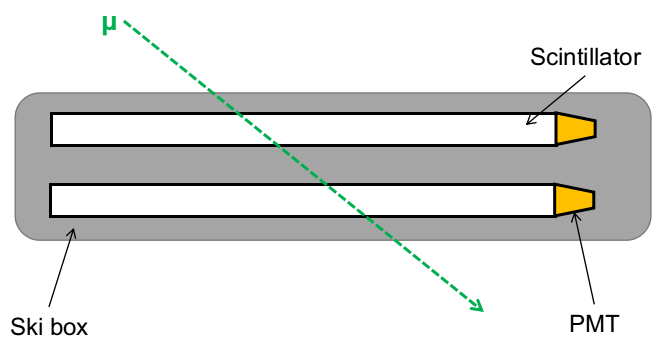
\includegraphics[width=0.75\columnwidth]{14008_config.png}
	\caption{Schematic diagram of the HiSPARC station 14008 detector set-up.}
	\label{fig:14008_config}
\end{figure}

To protect the scintillators and \glspl{pmt}, we sandwiched a layer of high density ($\rho = 38-40$~kg~m$^{-3}$, \citet{efoam_sf38_2017}) foam, of thickness, $\Delta x = 50$~mm, between the scintillators, as can be seen on the lab work bench in Figure~\ref{fig:14008_detectors}. Upon the completed assembly of the detectors, they are placed within the roof box on the roof of the Poynting Physics building on the campus of University of Birmingham, as shown in Figure~\ref{fig:14008_ski_box}.

\begin{figure}[ht!]
	\centering
	\subfloat[Scintillators on the work bench]{
		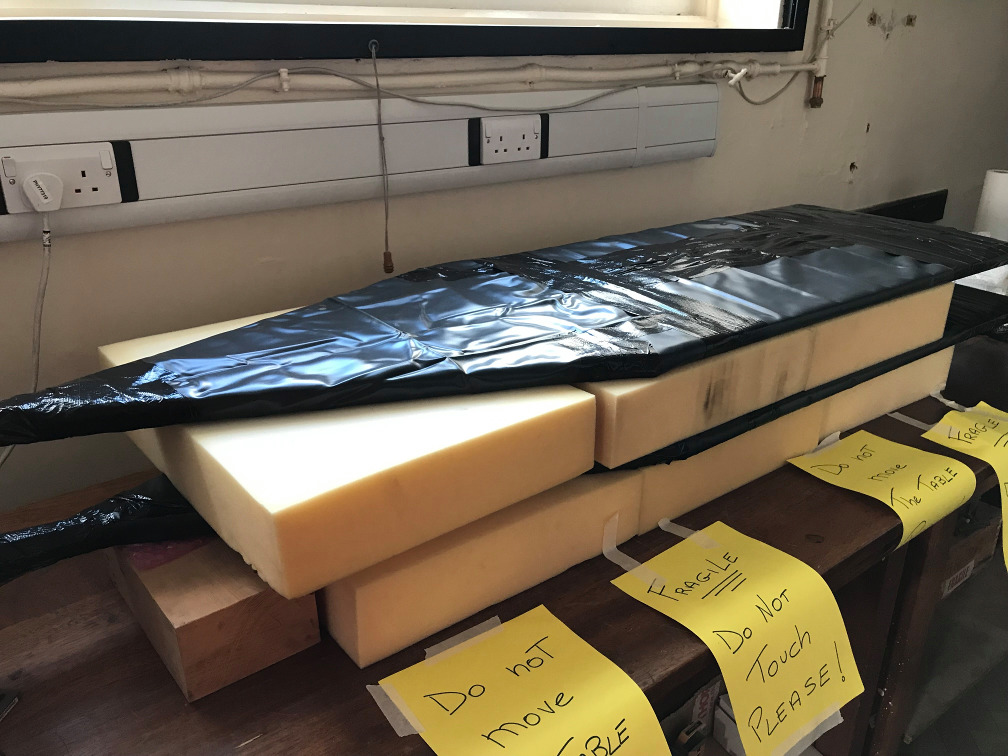
\includegraphics[width=0.48\columnwidth]{detectors_rescaled.jpg}
		\label{fig:14008_detectors}}
	%\qquad
	\subfloat[Complete detector on the roof]{
		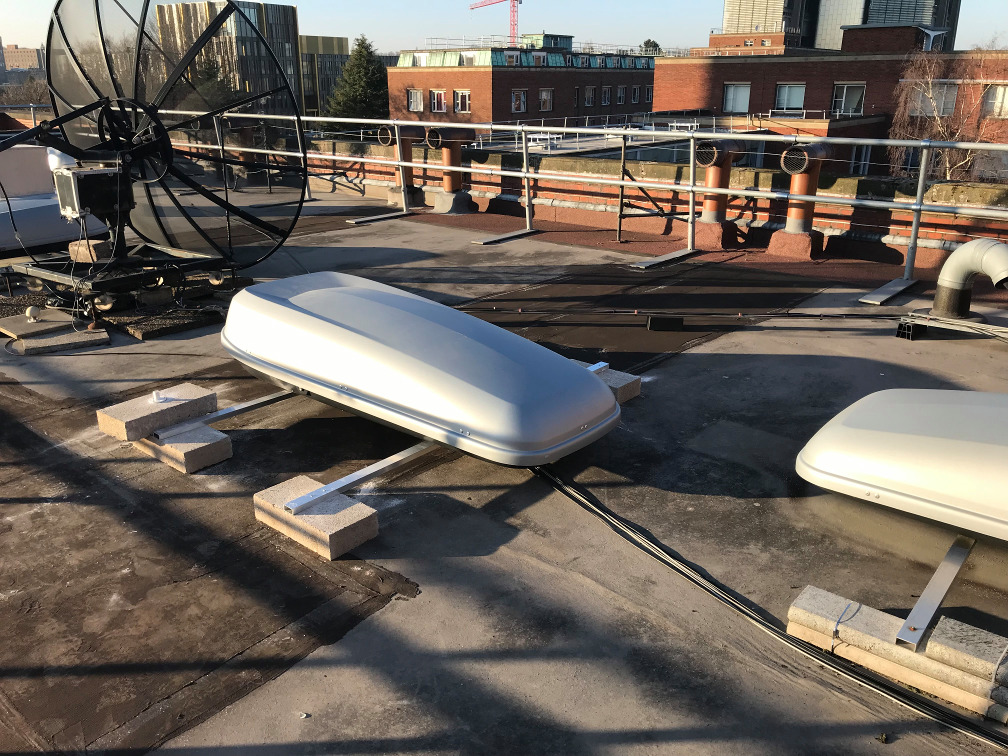
\includegraphics[width=0.48\columnwidth]{ski_box_rescaled.jpg}
		\label{fig:14008_ski_box}} \\
	
	\caption{HiSPARC 14008 assembly and configuration. (a) shows the stacked arrangement of the scintillators on the lab work bench, between layers of pretective foam. (b) shows the complete detector inside the roof box on the University of Birmingham campus.}
	\label{fig:HS_14008_setup}
\end{figure}


Propagating charged particles lose energy in matter. Derived from the Bethe-Bloch formula, we can estimate the amount of energy lost by a particle in a material given by:

\begin{equation}
\Delta E = \Delta x \, S \, \rho \, \cos(\theta) \, ,
\label{eq:energy_loss}
\end{equation}

where $\Delta x$ is the thickness of the material, $S$ is the stopping power of the material, $\rho$ is the density of the material, and $\theta$ is the angle the particle travels through the material from the perpendicular direction.

Each of the plastic scintillators has a thickness of $\Delta x \, = \, 2.0$~cm, and density, $\rho \, = \, 1.03$~g~cm$^{-3}$ \citep{montanus_observability_2017}. The stopping power of the scintillator for a minimum ionising particle is $S \sim 2$~MeV~g$^{-1}$~cm$^{2}$ \citep{fokkema_hisparc_2012, montanus_observability_2017}. The energy loss of a vertically incident muon in a single detector is therefore $\Delta E \sim 4$~MeV. \cite{van_dam_hisparc_2020} states the most probable energy loss of a vertically incident muon in a single scintillator is $3.51$~MeV.

 Assuming a similar stopping power as above for the foam, the muons will lose an additional $\sim 0.4$~MeV. In the complete configuration as a muon traverses two scintillators and the foam, the estimated lower limit on the energy loss by muons in the detector is $\sim 7.42$~MeV.


The standard \gls{hisparc} station set-up is such that the \glspl{pmt} are connected to the \gls{hisparc} electronics box for data acquisition. In the standard configuration, the trigger rate of events is $\sim 1$~Hz. In this stacked configuration the trigger rate is significantly higher, $\sim 70$~Hz; hence the data produced is the equivalent of approximately half of the existing \gls{hisparc} network. The network could not cope with such a large quantity of data, therefore we had to reduce the data acquired by the \gls{hisparc} box; however, we did not want to lose the full count rate of the stack detectors. To acquire the data in this set-up, we used a \gls{nim} crate, as shown in Figure~\ref{fig:14008_NIM}.

\begin{figure}[ht!]
	\centering
	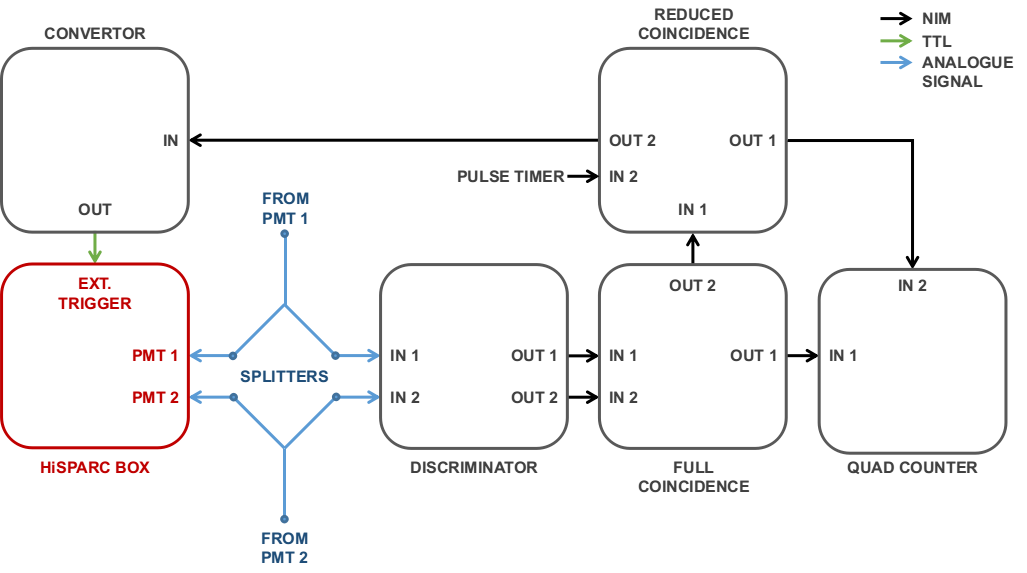
\includegraphics[width=\columnwidth]{14008_nim_config.png}
	\caption{Schematic diagram of the HiSPARC 14008 station's NIM crate configuration. Black arrows depict a NIM signal; green arrows show a TTL signal; blue arrows depict a HV signal.}
	\label{fig:14008_NIM}
\end{figure}

The data acquisition is discussed in Section~\ref{sec:HS14008_data_acqusition}, but here we discuss the configuration of the \gls{nim} crate set-up. The \gls{hv} signal from the detector \glspl{pmt} are split using a passive, equal-split resistive splitter such that half the signal is passed to the \gls{hisparc} electronics box and half the signal is passed through the \gls{nim} crate. The signal which is passed through the \gls{nim} crate is first passed into a discriminator module (CAEN model N845) to only record signals that have an amplitude greater than the trigger threshold. Due to the equal-balance resistive splitter the \gls{hv} signal is reduced in amplitude by a factor of 2; we used a discriminator threshold of $-35$~mV, i.e. half of the \gls{hisparc} high threshold.

The discriminator outputs two \gls{nim} signals which are connected to the first coincidence module (LeCroy model 622). This records every coincidence between the two \glspl{pmt} and the output from this module is directed to a \gls{nim} quad counter/timer module (ORTEC model 974). One channel of the \gls{nim} counter records the full coincidences from the first coincidence module.

A second terminal in the coincidence module was used to record a reduced count rate. This used a pulse timer (CAEN model 2255B) to create a gate signal with a $\sim 1\%$ duty cycle (gate width = $45.0 \, \upmu\mathrm{s}$ and repeat period = $4.86$~ms). The coincidence between the full coincidence signal and the pulse timer gate ensures that the full count rate is reduced by a factor of $\sim 100$. One output from this coincidence module is passed to the \gls{nim} counter, where it counts the reduced coincidences. The second output from the coincidence module is directed through a \gls{nim}-to-\gls{ttl} convertor and the output from this is used as an external trigger signal to trigger the acquisition of data by the \gls{hisparc} electronics box. This acquires the counts directly from the \glspl{pmt}.

[discussion, and also probably use a table, to discuss the delays introduce by the NIM crate...]


%%%%%%%%%%%%%%%%%%%%%%%%%%%%%%%%%%%%%%%%%%%%%%%%%%%%%%%%%%%%%%%%%%%%%
\subsection{Calibration}

When setting up the HiSPARC station, it was required to set several operating parameters for the detectors and the HiSPARC electronics box. One such setting was the \gls{pmt} operating voltage. Each of the detector \glspl{pmt} needs to be powered with a high enough operating voltage such to provide an amplified signal, but not too high such as to over-amplify the noise.

In general, the \glspl{pmt} has an advised operating voltage of around 700~V \citep{fokkema_hisparc_2019}; however, best practise is to operate the \gls{pmt} at the plateu region, whereby the counts/voltage no longer increases. As can be seen from Figure~\ref{fig:PMT_cal}, neither of the \glspl{pmt} have clear plateau regions, hence there was no obvious \gls{pmt} set point.

The HiSPARC installation manual does, however, suggest to tune the \gls{pmt} voltages such that the singles rates for each detector meet the following criteria: singles rate of 100--130 Hz for signal above the high trigger threshold, and singles rate of $<$400 Hz for signal above the low trigger threshold \citep{fokkema_hisparc_2019}.

In order to calibrate the \glspl{pmt} to the correct level, we measured the singles rates above the high and low thresholds as a function of \gls{pmt} operating voltage, as is shown in Figure~\ref{fig:PMT_cal} [UPDATE THIS PLOT...!!!!]. The voltage calibration plot shows drastically the different performances one can get from different \glspl{pmt}, therefore it is necessary to treat each \gls{pmt} individually when calibrating.

\begin{figure}[ht!]
	\centering
	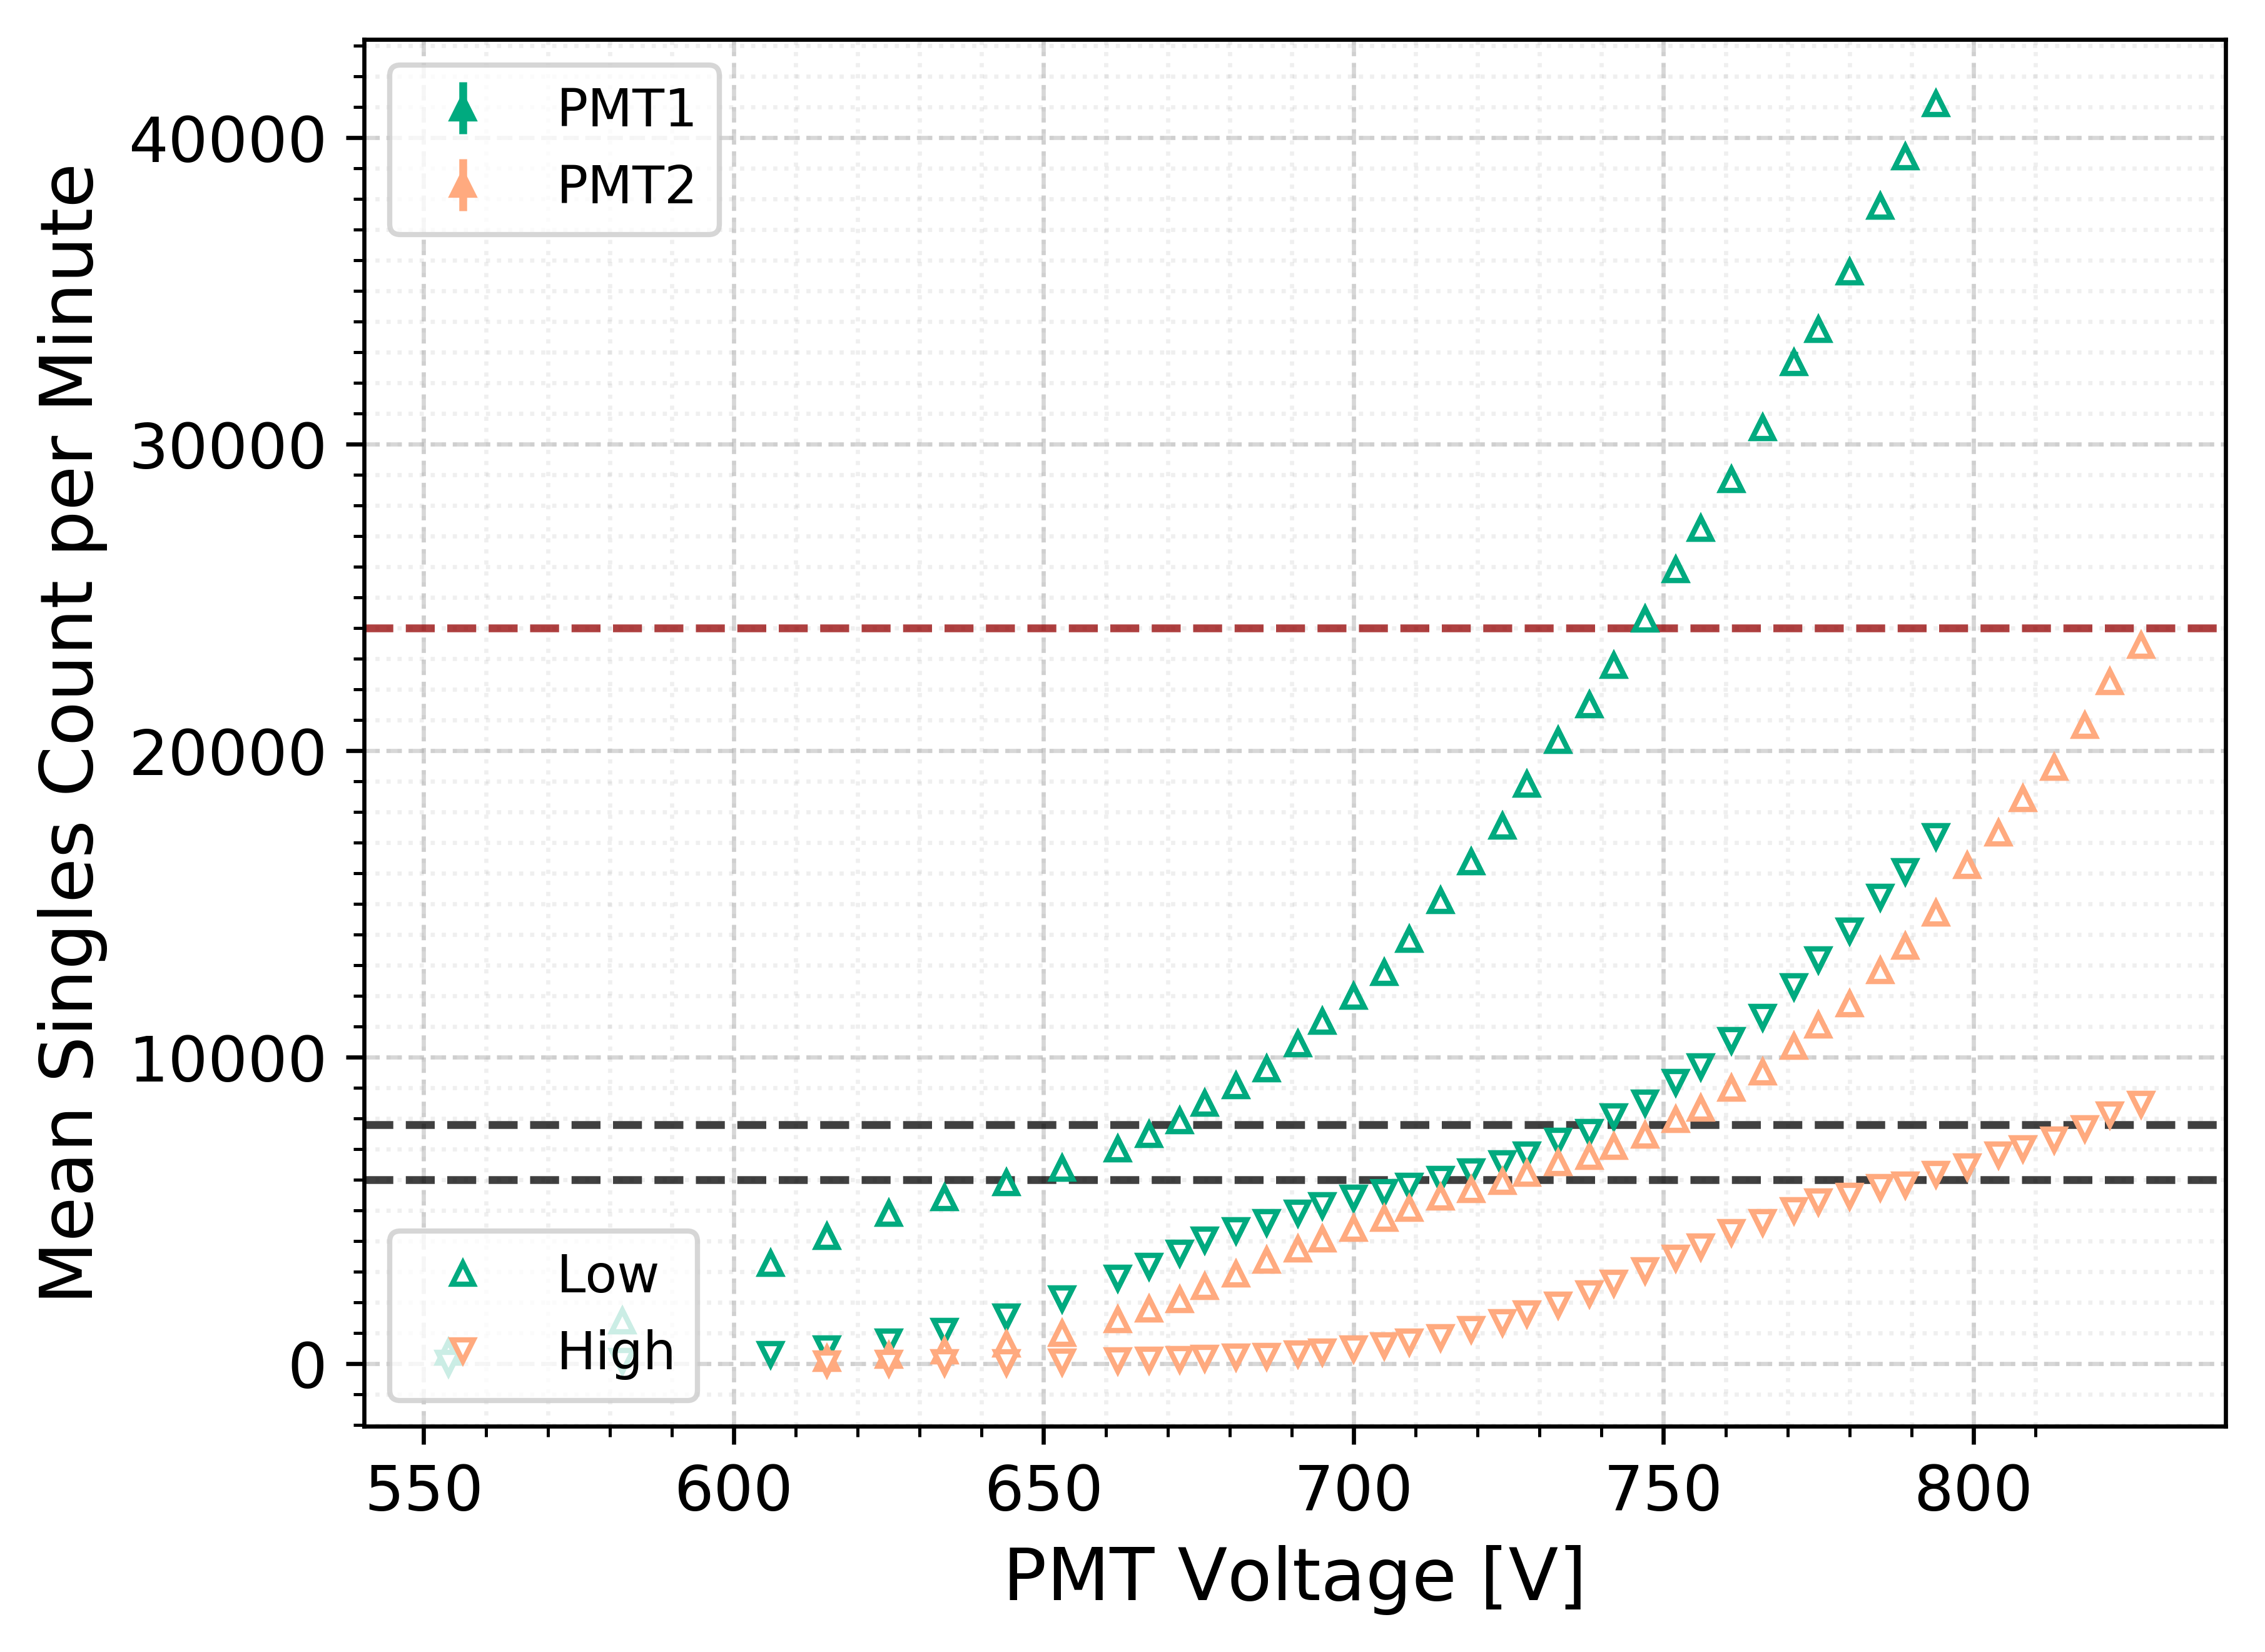
\includegraphics[width=0.8\columnwidth]{both_PMTs_post_NIM.png}
	\caption{Voltage calibration curve for the PMTs of station 14008. The upper, red-dashed line indicates the upper limit for the low threshold singles rate (400 Hz), and the lower 2, black-dashed lines indicate the upper and lower bounds for the high threshold singles rate (100--130 Hz).}
	\label{fig:PMT_cal}
\end{figure}




%%%%%%%%%%%%%%%%%%%%%%%%%%%%%%%%%%%%%%%%%%%%%%%%%%%%%%%%%%%%%%%%%%%%%
\subsection{Monitoring Temperature}

In Chapter~\ref{chap:HiSPARC}, we suspected that the singles count rates (and thus event count rates also) were affected by the temperature of the \gls{pmt} within the HiSPARC roof-boxes.

Some of the existing HiSPARC stations monitor local temperature however none measure the temperature of the \gls{pmt} within the roof box; therefore the temperature of the PMT itself is unknown, and thus we cannot account for the thermal noise. When building this new HiSPARC station, a temperature sensor was placed into the roof box which allowed us to monitor the temperature.

Figure~\ref{fig:temperature_sensor_circuit} shows the schematic for the temperature sensor. We used the DS18B20 temperature sensor with the one-wire telemetry protocol, which used a single wire to transmit the temperature readings to the microcontroller; the microcontroller used was a Raspberry Pi 4 (see Section~\ref{sec:HS14008_data_acqusition}). Three wires were used for the operation of the DS18B20: constant current voltage, ground, and data. The temperature is read on a 10-second cadence and is recorded in degrees Celsius with a precision of $0.001^{\circ}$~C. 

\begin{figure}[ht!]
	\centering
	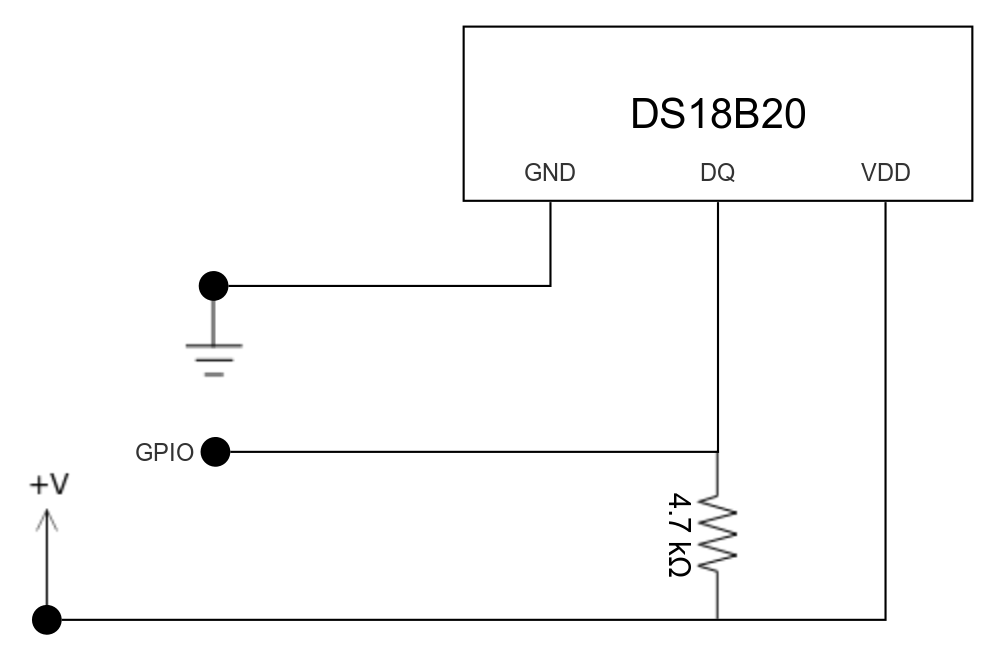
\includegraphics[width=0.6\columnwidth]{HS_14008_temp_circuit.png}
	\caption{Schematic diagram of the DS18B20 temperature sensor circuit, whereby the voltage, ground, and GPIO interfaces connect directly into pins of the Raspberry Pi board.}
	\label{fig:temperature_sensor_circuit}
\end{figure}




%%%%%%%%%%%%%%%%%%%%%%%%%%%%%%%%%%%%%%%%%%%%%%%%%%%%%%%%%%%%%%%%%%%%%
\subsection{Data Acquisition}
\label{sec:HS14008_data_acqusition}

The new \gls{hisparc} station uses two methods of data acquisition. The singles data and reduced coincidences data are acquired using the typical \gls{hisparc} data acquisition software, but the full coincidences, reduced coincidences, and the temperature data are all acquired by a Raspberry Pi 4. This was done as it allowed us to store the full coincidences data. A schematic diagram showing the interfaces between the Raspberry Pi and the other hardware is shown in Figure~\ref{fig:14008_RP4}.

\begin{figure}[ht!]
	\center
	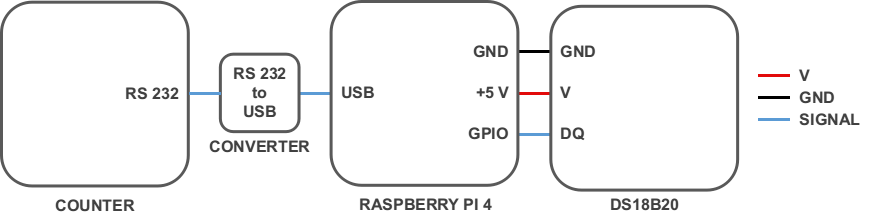
\includegraphics[width=0.8\columnwidth]{14008_data_acq_config.png}
	\caption{Schematic diagram of the HiSPARC station 14008 data acquisition interfaces.}
	\label{fig:14008_RP4}
\end{figure}


The Raspberry Pi 4 was used to control the data acquisition by running a Python script. The scripts configured the hardware and output the coincidences data from the \gls{nim} counter and the temperature data from the DS18B20 sensor to local files on the Raspberry Pi. Both the coincidences and temperature data are recorded on a 10 second cadence.

Each new day generates a separate file for the coincidences data and temperature data. Within the coincidence files there are no headers and the data begins from line 1. The files contain four columns and the data stored in each column is listed in Table~\ref{tab:HS_14008_coincidences_data}.

\begin{table}[ht!]
	\begin{center}
		\caption{Variables stored in the coincidences files of the HiSPARC 14008 instrument.}
		\label{tab:HS_14008_coincidences_data}
		\begin{tabular}{cp{0.2\linewidth} lp{0.35\linewidth} cp{0.3\linewidth} cp{0.35\linewidth}}
			\hline 
			{\bf Column} & {\bf Item} & {\bf Unit} & {\bf Type} \\ 
			\hline 
			\multirow{2}*{0} & \multirow{2}*{Time Stamp} & YYYY\_MM\_DD & \multirow{2}*{String}  \\ 
			  &  & HH:MM:SS.ffffff & \\ 
			1 & Time*  & Decisecond & Integer, eight digits, zero padded \\ 
			2 & Cumulative Reduced Count* & Counts & Integer, eight digits, zero padded \\ 
			3 & Cumulative Full Count* & Counts & Integer, eight digits, zero padded \\ 
			\hline 
		\end{tabular} 
	\end{center}
	* Since restart
\end{table}

The \gls{nim} counter records the cumulative coincidences count, therefore the reduced and full data stored are also cumulative and thus when reading the data, one must ensure that the difference is calculated between timestamps. In the event of hardware or software failure, or a reboot of the Raspberry Pi, when the Python script re-runs the \gls{nim} counter restarts all values from 0. When reading a file, one must ensure that checks are in place to handle any restarts from zero appropriately, such that no negative counts are calculated from one timestamp to the next during a restart.

Within the temperature files, there are also no headers and the data begins from line 1. The columns in the data file are outlined in Table~\ref{tab:HS_14008_temperature_data}.

\begin{table}[ht!]
	\begin{center}
		\caption{Variables stored in the temperature files of the HiSPARC 14008 instrument.}
		\label{tab:HS_14008_temperature_data}
		\begin{tabular}{c l l l}
			\hline 
			{\bf Column} & {\bf Item} & {\bf Unit} & {\bf Type} \\ 
			\hline 
			\multirow{2}*{0} & \multirow{2}*{Time Stamp} & YYYY\_MM\_DD & \multirow{2}*{String}  \\ 
			  &  & HH:MM:SS.ffffff & \\ 
			1 & Temperature & $^\circ$C & Floating point \\ 
			\hline 
		\end{tabular} 
	\end{center}
\end{table}


The data is stored locally, but it is also stored on the University of Birmingham particle physics servers as a back-up\footnote{Disk location: /disk/moose/general/epesv001/datadisk/147.188.46.117\_hisparc\_pi/}. Access to the data is not necessarily open, and to request access, one should contact the System Administrator for the Particle Physics Group Computing Facilities.

The reduced coincidences data are acquired using the \gls{hisparc} data acquisition software and are stored within the \gls{hisparc} servers. The \gls{hisparc} servers record this data as the events and the data can be acquired using the methods described in Section~\ref{sec:HS_data}.




[What is the width of the signals generated by the NIM crate? Is it more or less than the approx. 25ns FWHM of the pulses..? Then relate that to: "The pulse width, Tw, is important only insofar as it determines the maximum rate of pulses that may be represented by the pulse train, since pulses which occur more frequently than 1/Tw cannot be resolved"...]



[a few statements on the availability of the data... i.e. it's generally ok and a complete set beyond Feb 2020, but many interruptions due to the pandemic... After around Sept 2020 the data becomes more reliable...]



%%%%%%%%%%%%%%%%%%%%%%%%%%%%%%%%%%%%%%%%%%%%%%%%%%%%%%%%%%%%%%%%%%%%%
\subsection{Monitoring Pressure}

As with the previous chapter, it was still necessary to account for the barometric effect on the muon count rate, for both the singles data and the full and reduced coincidences data. To monitor the pressure, a nearby station was used, which is part of the \gls{midas} database, and acquired from the \gls{stfc} and \gls{nerc} \gls{ceda} archive.

The \gls{midas} station used is the nearest pressure monitor to the \gls{hisparc} and provides a robust measure of the local atmospheric pressure. The pressure is measured at the \gls{midas} station level and a correction for altitude is not applied. The station is located in Coleshill, Warickshire (ID: 19187), nearby Birmingham International Airport, $\sim 20$~km from the HiSPARC detectors; we believe the pressure variation is small over this distance.

The pressure data is recorded on a 1-hour cadence in units of hPa, with a precision of 0.1~hPa. The time variation of pressure is slow; hence, we linearly interpolated the data to provide a 1-minute sample.


%%%%%%%%%%%%%%%%%%%%%%%%%%%%%%%%%%%%%%%%%%%%%%%%%%%%%%%%%%%%%%%%%%%%%
%%%%%%%%%%%%%%%%%%%%%%%%%%%%%%%%%%%%%%%%%%%%%%%%%%%%%%%%%%%%%%%%%%%%%
\section{Methodology}\label{sec:HS_14008_methods}

\subsection{Atmospheric Corrections}

Using the theory outlined in Section~\ref{sec:HS_P_corr} we were able to perform the barometric correction of the singles data and coincidences data...

Method of temperature correction is using the linear relationship. Steps are:

- first remove the long term temperature trend over a month of data, done by smoothing the singles and temperature data using a 24-hr box-car , and removing the long term, covariance

- second, after removing the long term trend, for each day the temperature correction is applied again to remove the daily variations...



\subsection{Observations}

[discuss statistics of observations, i.e. follow poisson and poisson is additive...]

The probability distribution of the number of counts in a fixed interval of time follows the Poisson distribution and is defined by:

\begin{equation}
P(k; \lambda) = \frac{\lambda^k \exp{-\lambda}}{k!} \, ,
\end{equation}
%
where $k$ is the number of events, which is always an integer, and $\lambda$ is the mean value of the number of events per interval, i.e. the expected number.

The Poisson distribution is also additive such that...



[discuss simulations and statistics tests...]


%%%%%%%%%%%%%%%%%%%%%%%%%%%%%%%%%%%%%%%%%%%%%%%%%%%%%%%%%%%%%%%%%%%%%
%%%%%%%%%%%%%%%%%%%%%%%%%%%%%%%%%%%%%%%%%%%%%%%%%%%%%%%%%%%%%%%%%%%%%
\section{Atmospheric Corrections}\label{sec:HS_14008_atmospheric_correction}

%%%%%%%%%%%%%%%%%%%%%%%%%%%%%%%%%%%%%%%%%%%%%%%%%%%%%%%%%%%%%%%%%%%%%
\subsection{Barometric Correction}\label{sec:HS_14008_P_corr}


Using the theory outlined in Section~\ref{sec:HS_P_corr} we were able to perform the barometric correction between the 1-minute interpolated pressure data and 1-minute averaged coincidences and singles data.

[show the plot of the correction over a month...]


\begin{figure}[ht!]
	\centering
	\subfloat[...]{
		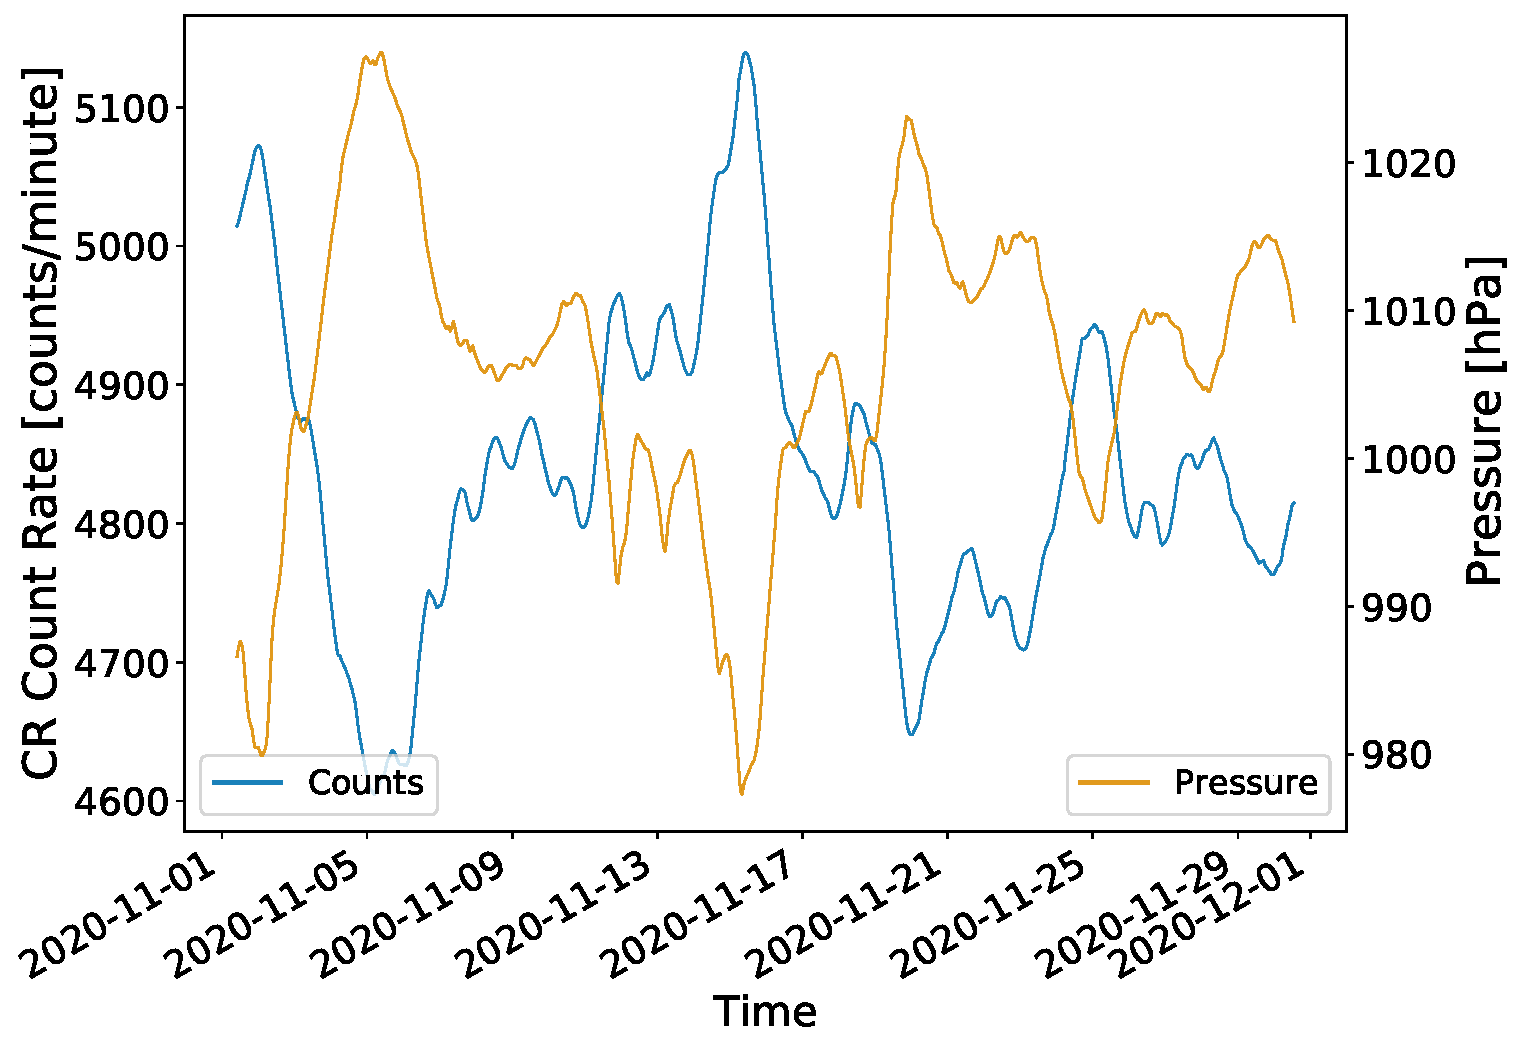
\includegraphics[width=0.48\columnwidth]{CR_v_P.pdf}
		\label{fig:HS_14008_CRvP}}
	%\qquad
	\subfloat[Correlation between singles and pressure]{
		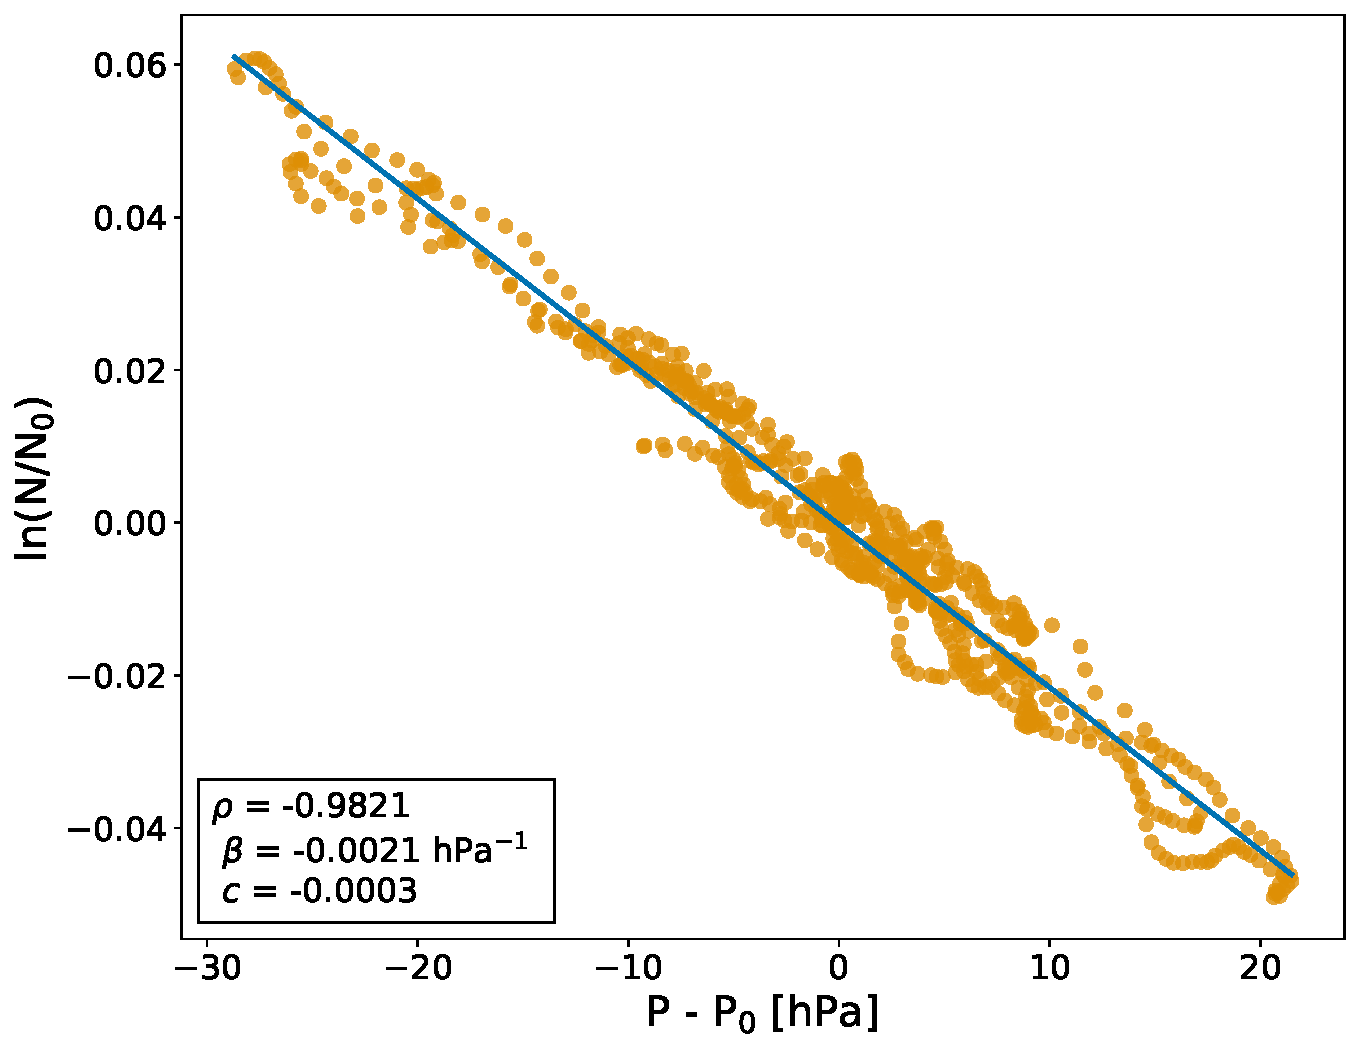
\includegraphics[width=0.48\columnwidth]{fit_CR_v_P.pdf}
		\label{fig:HS_14008_beta}} \\
	
	\caption{The relationship between the ... (a) shows the ... and pressure data; (b) shows the correlation between the singles counts and pressure, and the fitted line to calculate the correction coefficient.}
	\label{fig:14008_CR_V_P_corr}
\end{figure}


[show a before vs after plot too...]


\begin{figure}[ht!]
	\centering
	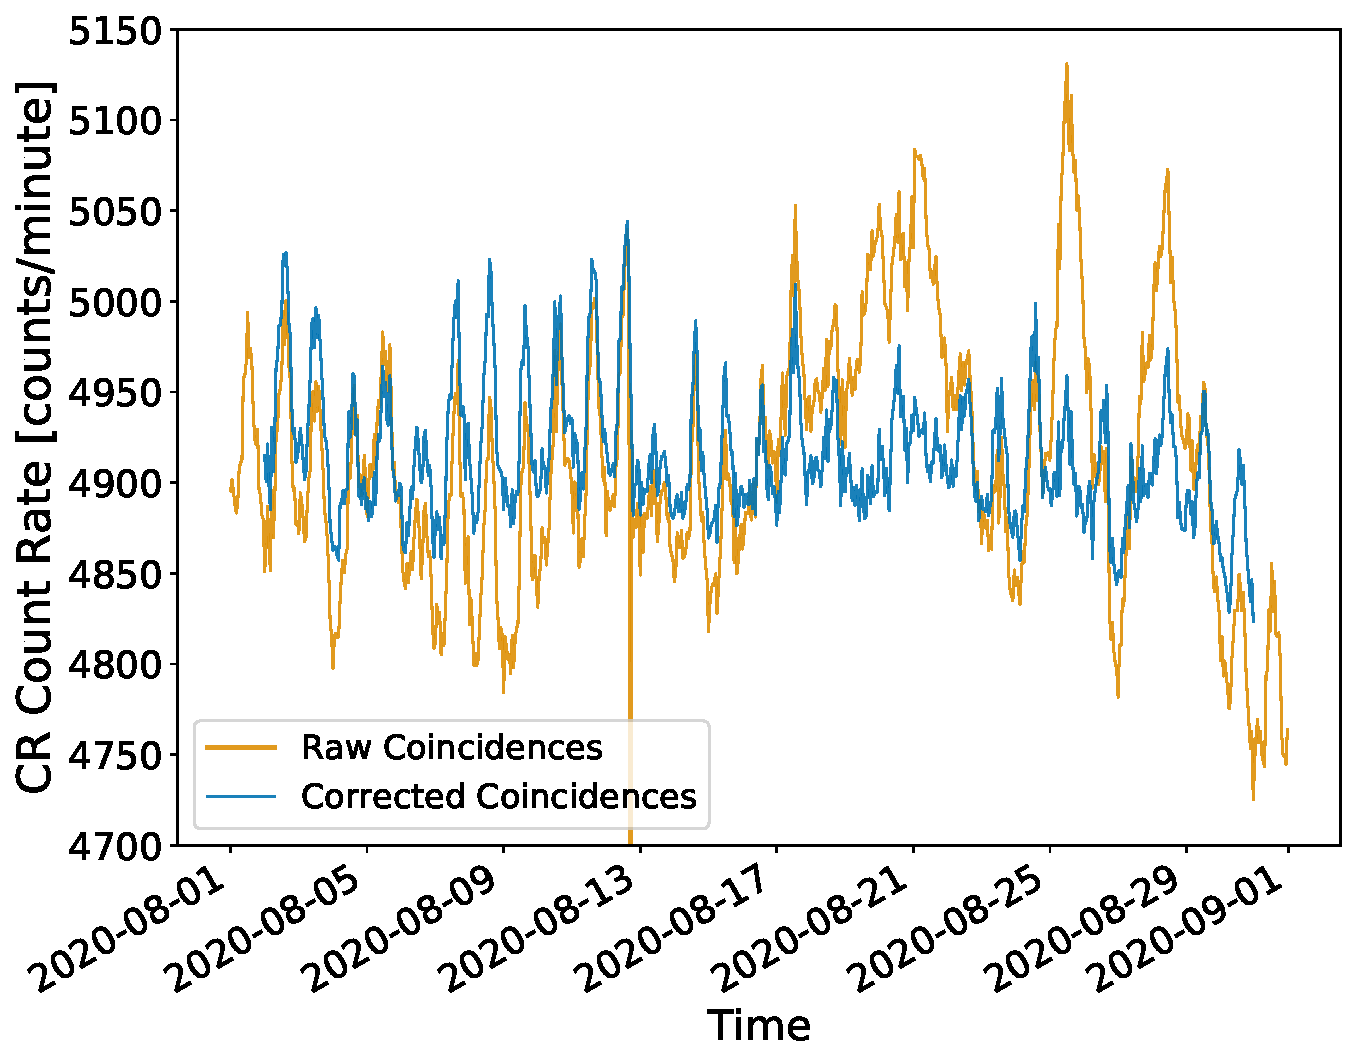
\includegraphics[width=0.75\columnwidth]{raw_vs_corrected_coincidences.pdf}
	\caption{...}
	\label{fig:HS_14008_corrected_coincidences}
\end{figure}



%%%%%%%%%%%%%%%%%%%%%%%%%%%%%%%%%%%%%%%%%%%%%%%%%%%%%%%%%%%%%%%%%%%%%
\subsection{Temperature Correction}\label{sec:HS_14008_T_corr}

One can see the relationship between the singles rates and the temperature in Figure~\ref{fig:HS_14008_temperature_vs_CR}...

\begin{figure}[ht!]
	\centering
	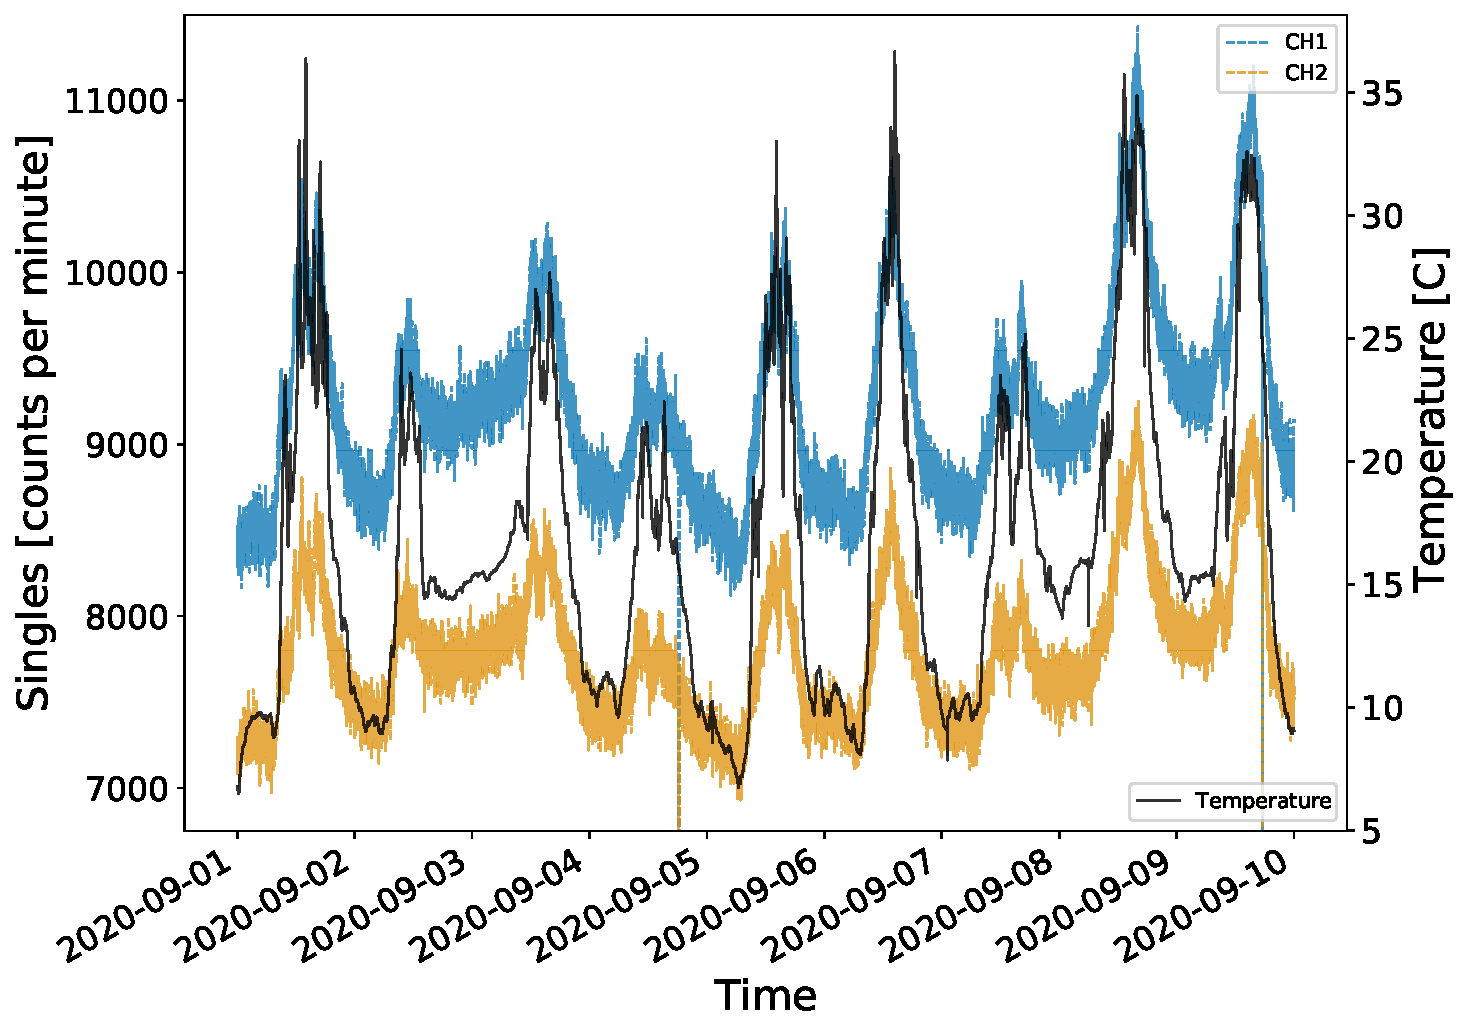
\includegraphics[width=0.75\columnwidth]{HS_14008_CR_v_T_sept2020.pdf}
	\caption{...}
	\label{fig:HS_14008_temperature_vs_CR}
\end{figure}




\begin{figure}[ht!]
	\centering
	\subfloat[...]{
		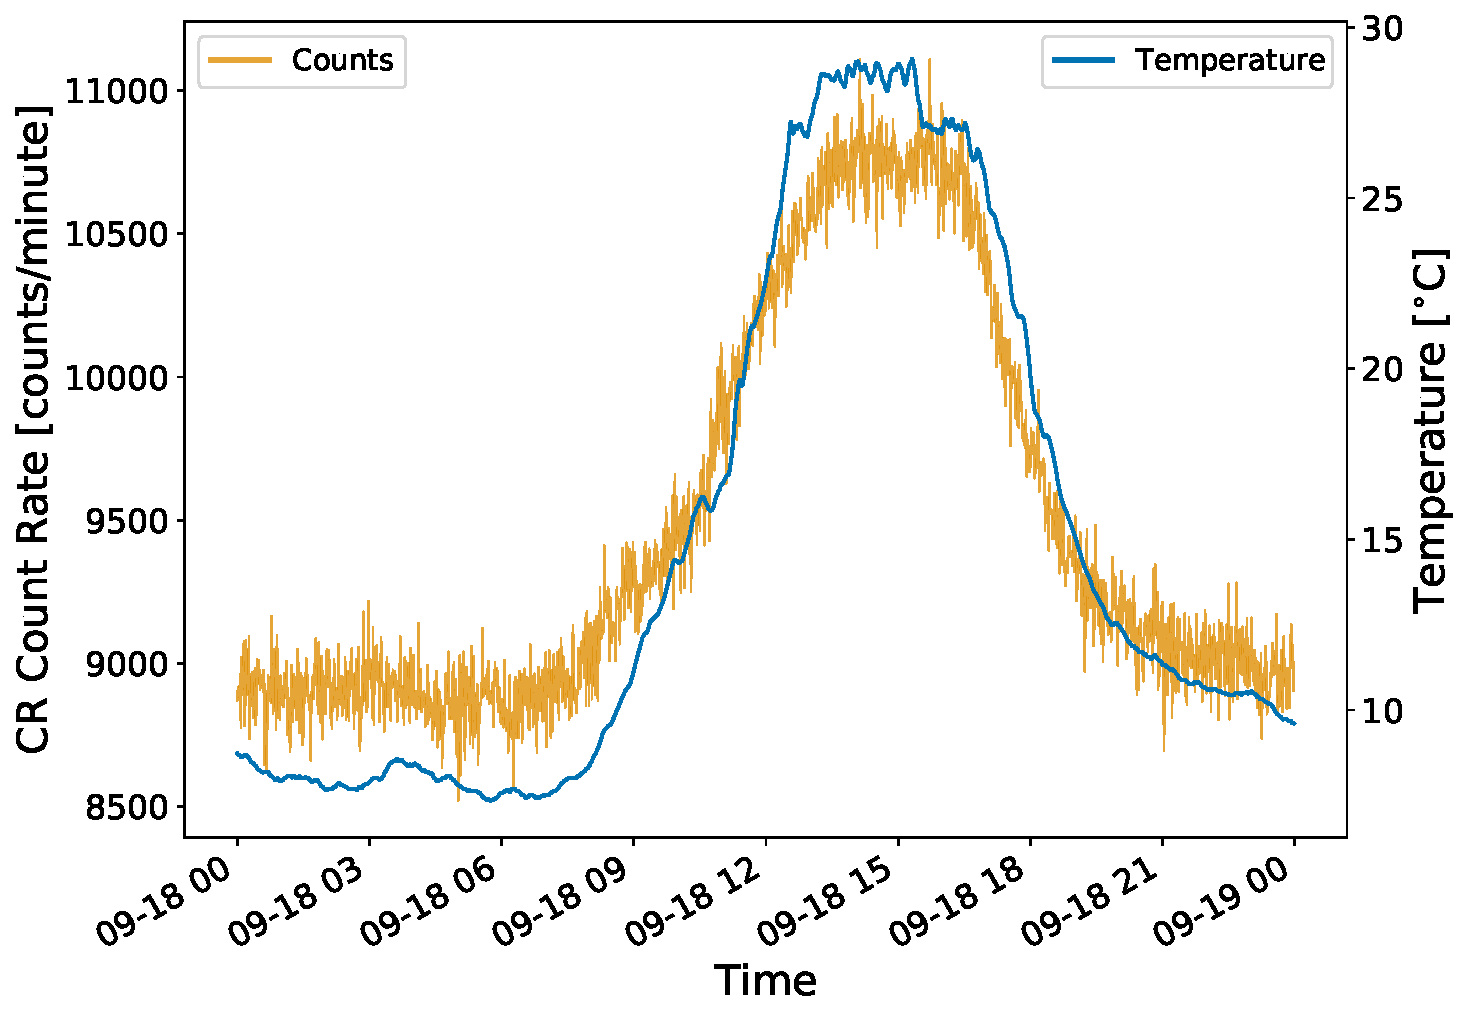
\includegraphics[width=0.48\columnwidth]{CR_v_T.pdf}
		\label{fig:HS_14008_CRvT}}
	%\qquad
	\subfloat[Correlation between singles and temperature]{
		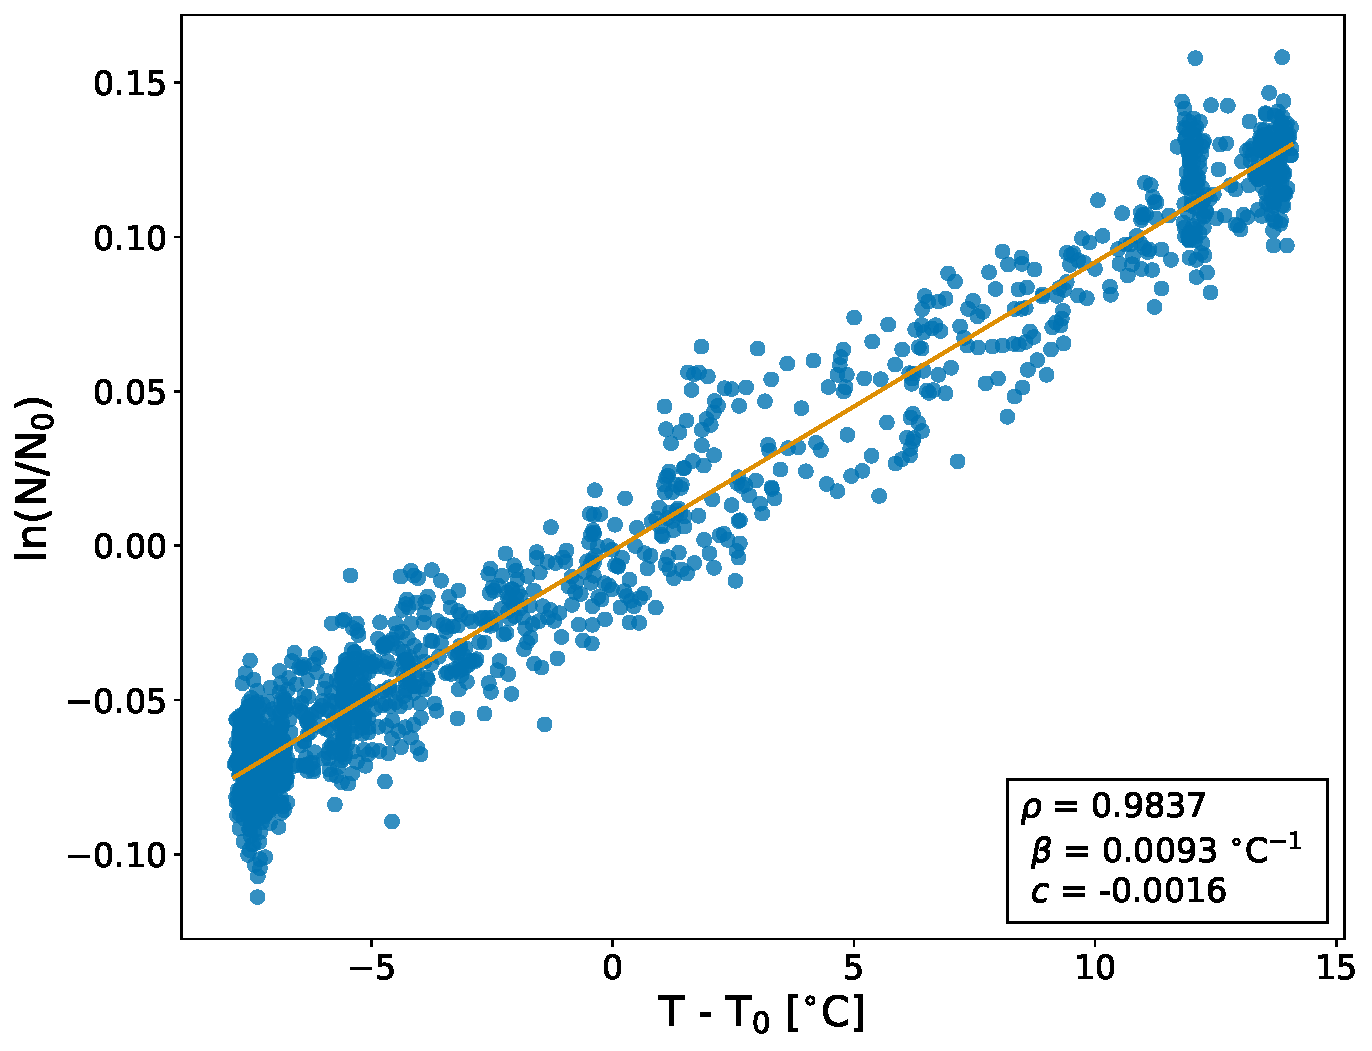
\includegraphics[width=0.48\columnwidth]{fit_CR_v_T.pdf}
		\label{fig:HS_14008_alpha}} \\
	
	\caption{The relationship between the ... (a) shows the ... and temperature data; (b) shows the correlation between the singles counts and temperature, and the fitted line to calculate the correction coefficient.}
	\label{fig:14008_CR_V_T_corr}
\end{figure}


An additional benefit of the temperature monitor at station 14008 is that it is suitable for providing an estimate of the temperature inside the roof-boxes of stations 14001, which is located on the same roof.... [show figure of the singles for both stations and the temperature!]


[Note: temperature correction doesn't work/not necessary on the coincidences but it is necessary on the singles rates!]





%%%%%%%%%%%%%%%%%%%%%%%%%%%%%%%%%%%%%%%%%%%%%%%%%%%%%%%%%%%%%%%%%%%%%
%%%%%%%%%%%%%%%%%%%%%%%%%%%%%%%%%%%%%%%%%%%%%%%%%%%%%%%%%%%%%%%%%%%%%
\section{Results}\label{sec:HS_14008_observations}

%%%%%%%%%%%%%%%%%%%%%%%%%%%%%%%%%%%%%%%%%%%%%%%%%%%%%%%%%%%%%%%%%%%%%
%%%%%%%%%%%%%%%%%%%%%%%%%%%%%%%%%%%%%%%%%%%%%%%%%%%%%%%%%%%%%%%%%%%%%
\subsection{Observations}\label{sec:HS_14008_observations}

From the \gls{corsika} simulations in Chapter~\ref{chap:HiSPARC}, we predicted a ground level muon rate passing through a single \gls{hisparc} detector of $\sim 85 \, \upmu/\mathrm{s}$ (for non-vertical, i.e. $70^\circ$ acceptance cone simulations), and $160 \, \upmu/\mathrm{s}$ (for vertical simulations). These rates were comparable to the generally accepted, average ground level muon flux on the order of $\sim 70 \, \mathrm{m}^{-2}\,\mathrm{s}^{-1}\,\mathrm{sr}^{-1}$ \citep{cecchini_cosmic_2000, blackmore_terrestrial_2015, pereira_ground_2020, particle_data_group_review_2020}.

%(do this by intergrating under curve, using 70-degre half-angle cone for solid angle, and area of 0.5m2)
% i.e. in python doing doing:
% where df contains the alpha and proton diff fluxes
% v = scipy.integrate.simps(df_a_v[1]+df_p_v[1], df_a_v.index.values)
% sr = 4*np.pi*(np.sin(np.deg2rad(70/2)))**2
% area = 0.5
% rate_v = v*sr*area

In Figure~\ref{fig:corrected_coinciences} we show the full coincidence count for a typical day. In this plot we can see the diurnal effect. The diurnal effect measured here induced a variation in the \gls{cr} count between $\sim 1-2 \%$, which is larger than the $\sim 0.5 \%$ diurnal variation, discussed in the literature \citep{mishra_study_2007, mishra_cosmic_2008, dubey_cosmic_2016, thomas_decadal_2017}, but is significantly lower than the variation observed in the \gls{hisparc} events and singles data in Chapter~\ref{chap:HiSPARC}. For any given epoch, the diurnal effect can be removed, if necessary, by removing the trend of a 12-hour smoothed data set, which is also shown in Figure~\ref{fig:corrected_coinciences}.

\begin{figure}[ht!]
	\centering
	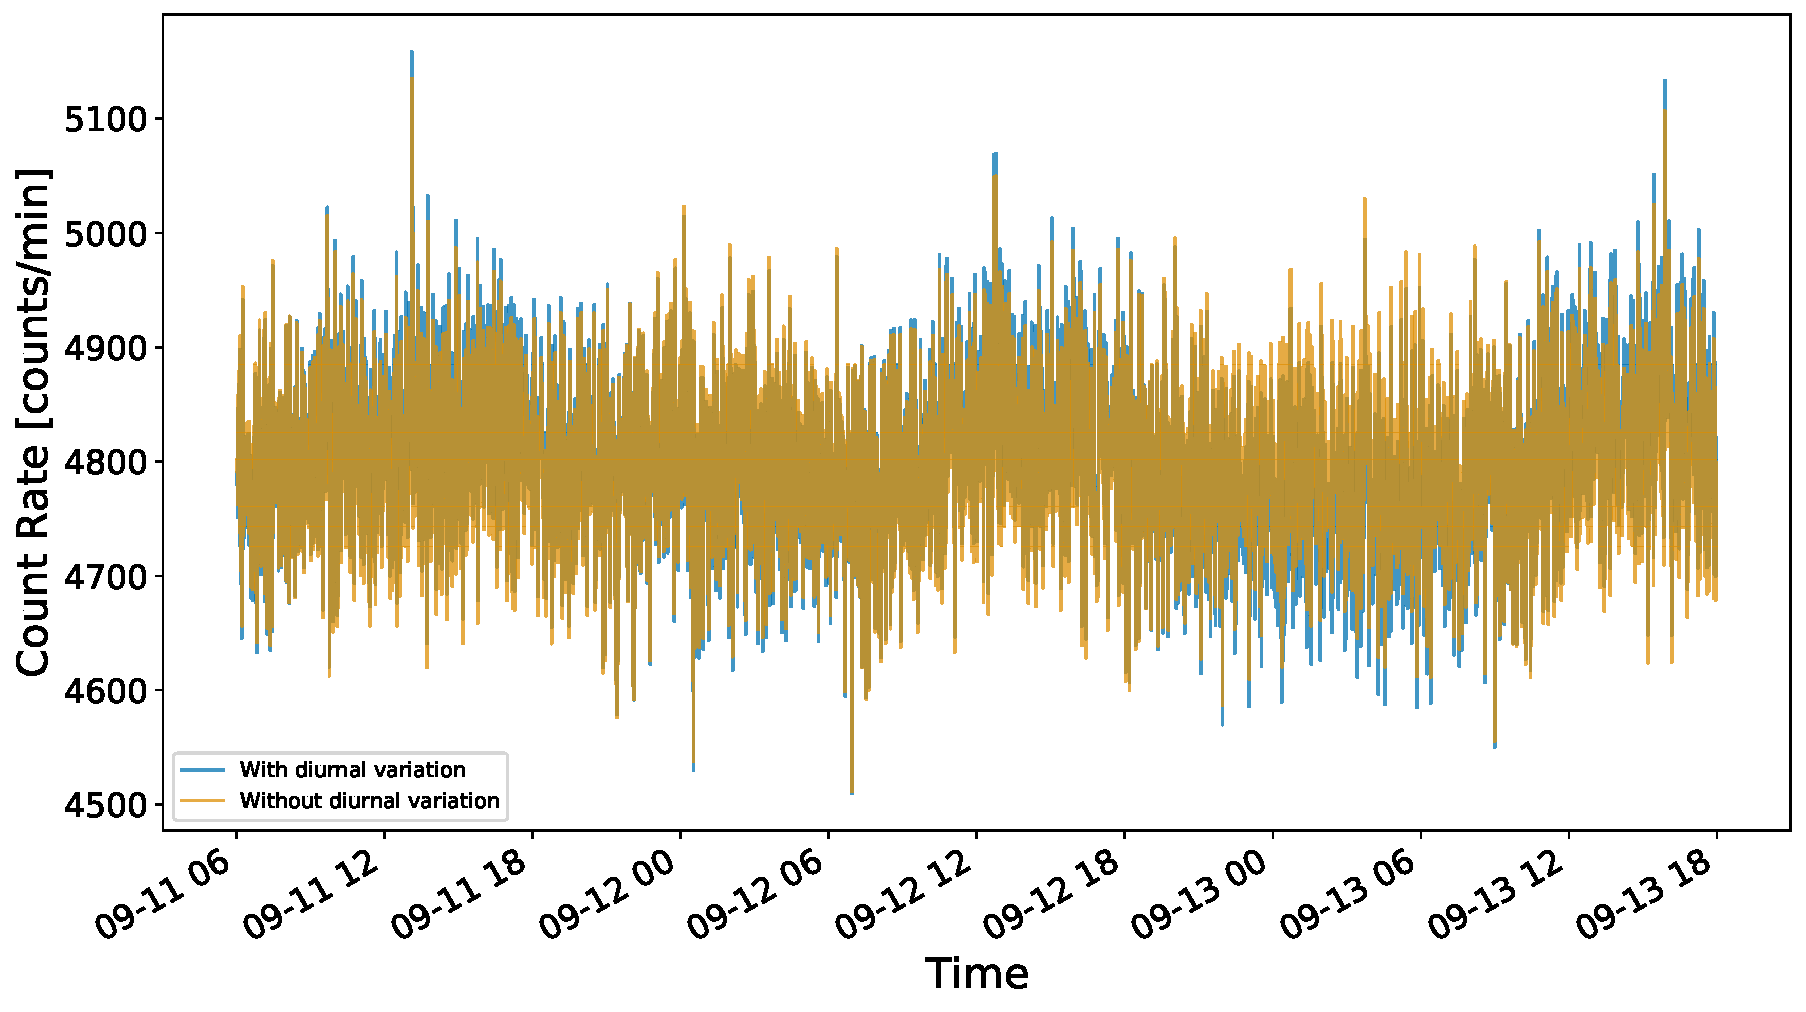
\includegraphics[width=\columnwidth]{many_day_diurnal_effect_timeseries.pdf}
	\caption{Time series of coincidences data, corrected for atmospheric pressure and displaying the diurnal variation with a peak at around midday.}
	\label{fig:corrected_coinciences}
\end{figure}


As the counts follow a Poisson distribution we sampled the data using the {\verb pymc3 } \gls{nuts} extension to a \gls{hmc} sampling algorithm \citep{salvatier_probabilistic_2016} with a Poisson distribution likelihood function. This allowed us to determine the mean count rate. Convergence was interrogated using the $\widehat{R}$ diagnostic factor using the criteria that chains did not converge if $\widehat{R} > 1.01$. 

%The distribution of the random coincidences is shown in Figure~\ref{fig:poisson_coinciences_dist}.
%
%
%\begin{figure}[ht!]
%	\centering
%	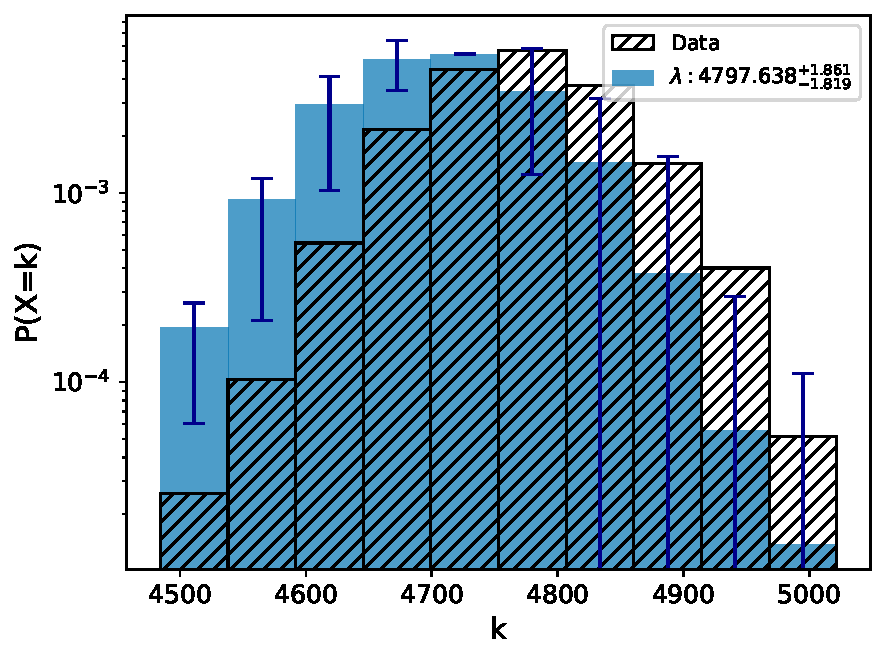
\includegraphics[width=0.9\columnwidth]{fitted_poisson.pdf}
%	\caption{Distribution of ... and Poisson distribution of the random coincidences, along with the median posterior fitted mean of the sample...}
%	\label{fig:poisson_coinciences_dist}
%\end{figure}


The median value of the posterior distribution for the mean value of the Poisson distribution of these coincidence data is $4797 \pm 2$~counts/min, where the uncertainties represent the $68 \%$ credible intervals either side of the median. We therefore have a count rate of $\sim 80 \, \upmu/\mathrm{s}$ in this stacked detector configuration. This is lower than the estimates predicted in the simulations in Chapter~\ref{chap:HiSPARC}, but is close to the predicted values for the non-vertical simulations, which represent a good approximation to the true muon flux at ground level. With a count rate of count rate of $\sim 80 \, \upmu/\mathrm{s}$, the Poisson noise is a rate of $\sim 9 \, \upmu/\mathrm{s}$, which represents $\sim 11 \%$ of the signal.


These observations have shown the full coincidences data, which are stored only locally. The data sent to the \gls{hisparc} servers are the reduced counts, which use the \gls{nim} gate signal to reduce the count rate by a factor of $\sim 100$. This data is also stored locally, but the data are acquired slightly differently. As discussed in Section~\ref{sec:HS14008_data_acqusition}, the reduced counts stored locally use the \gls{nim} counter to count the rate of the external trigger signal (i.e. coincidences between the \gls{nim} gate signal, and the coincidences between the two \glspl{pmt}). The \gls{hisparc} events data uses this trigger to read the events directly from the \glspl{pmt}. Due to the delays in the signal in the \gls{nim} create, one could reasonably have a concern that the two sources of data may differ. In Figure~\ref{fig:reduced_coincidences} we show a comparison between the reduced coincidences data stored locally and those recorded as events data in the \gls{hisparc} server.

%\begin{figure}[ht!]
%	\centering
%	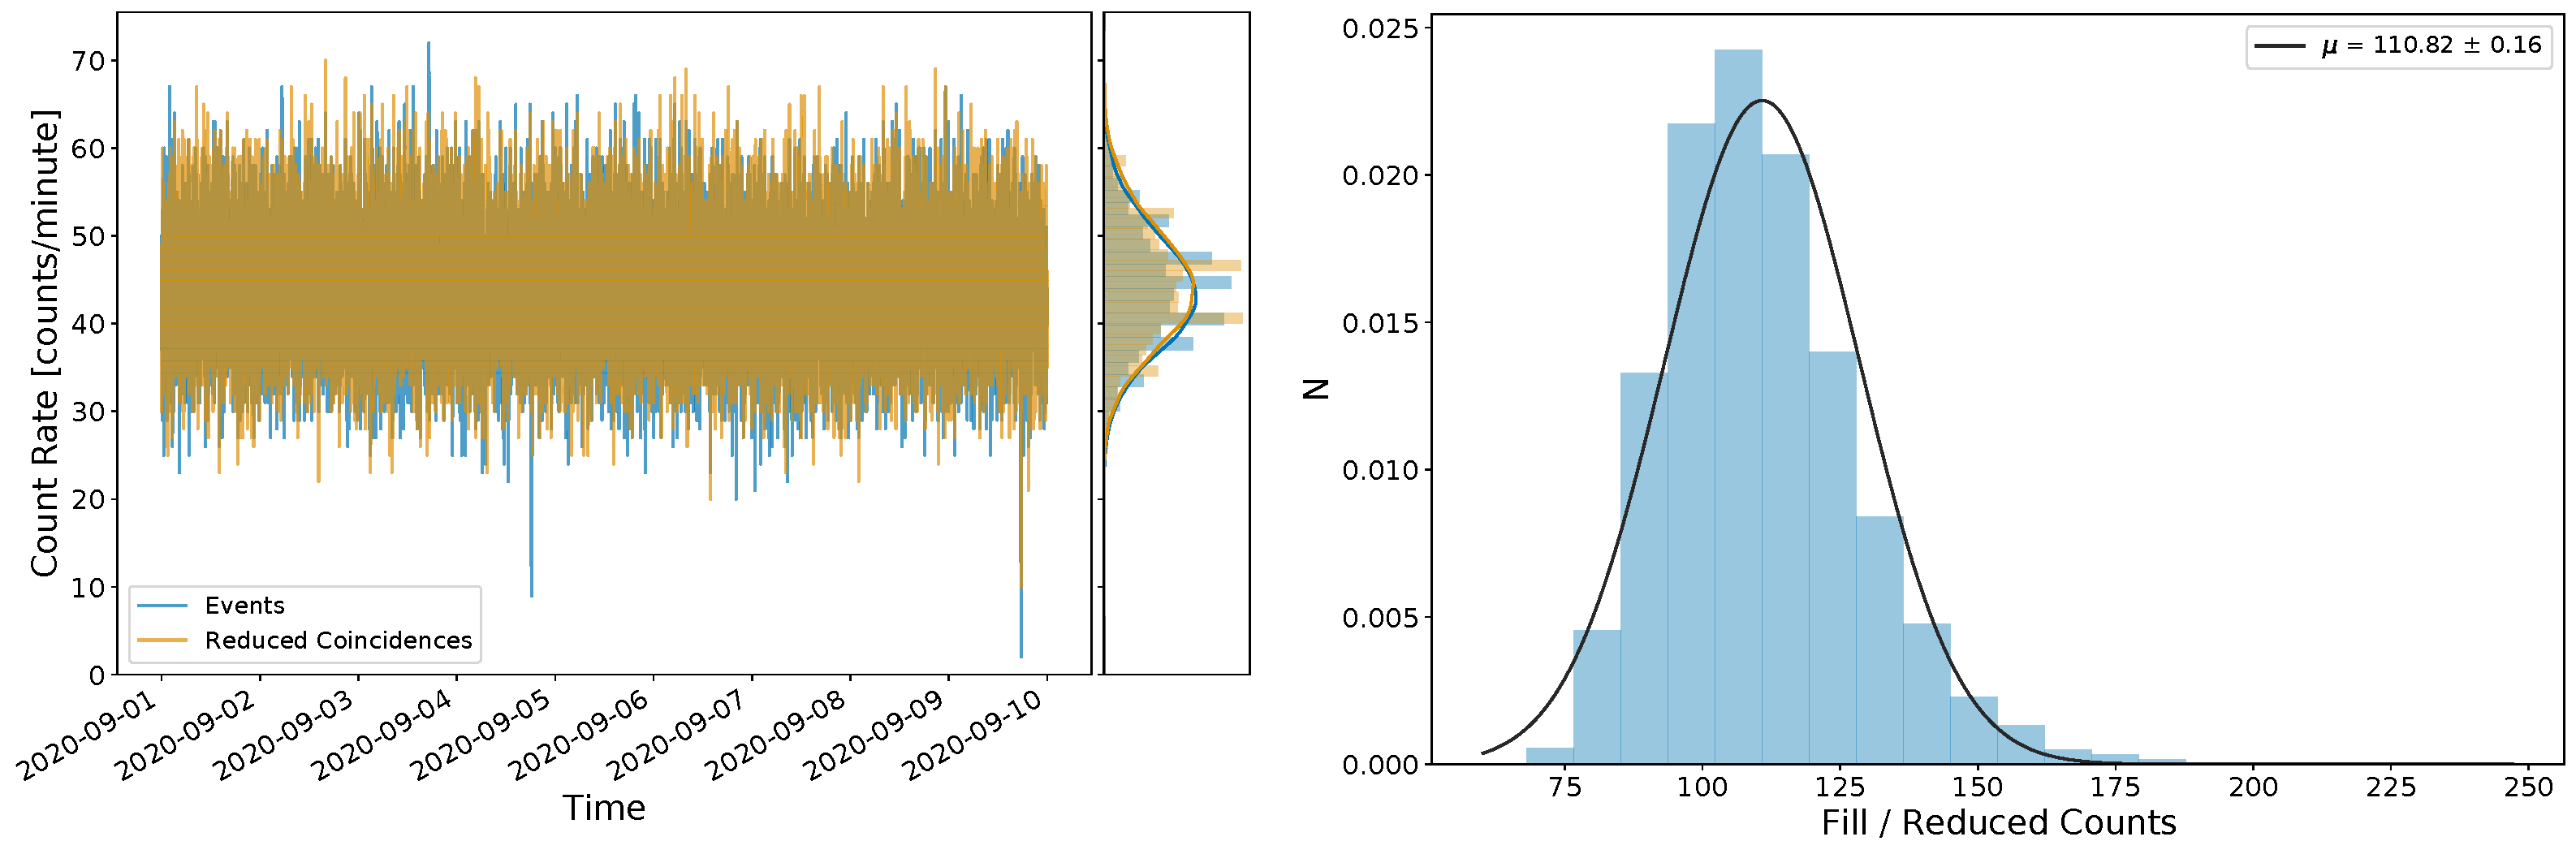
\includegraphics[width=\columnwidth]{reduced_coinc.pdf}
%	\caption{Comparison of the reduced coincidences stored locally and as events data in the HiSPARC server (left); }
%	\label{fig:reduced_coincidences}
%\end{figure}

\begin{figure}[ht!]
	\centering
	\subfloat[Timeseries of reduced coincidences]{
		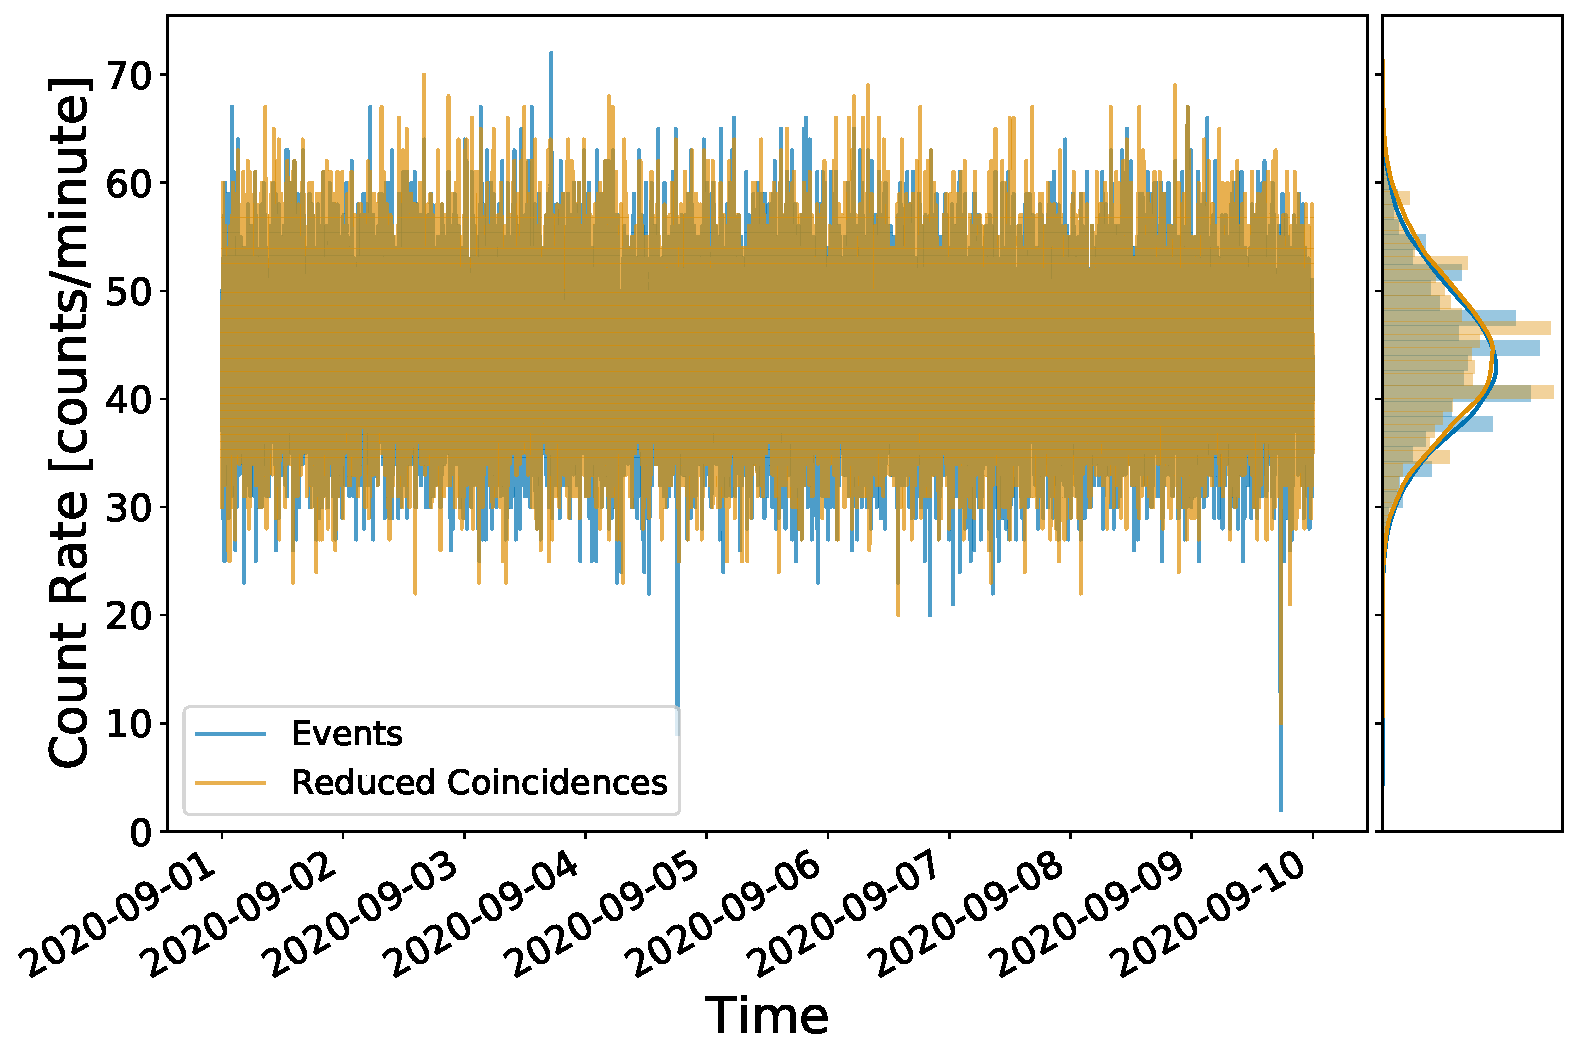
\includegraphics[width=0.52\columnwidth]{reduced_events_vs_coinc.pdf}
		\label{fig:rc1}}
	%\qquad
	\subfloat[Distribution of full-to-reduced coincicdences ratio]{
		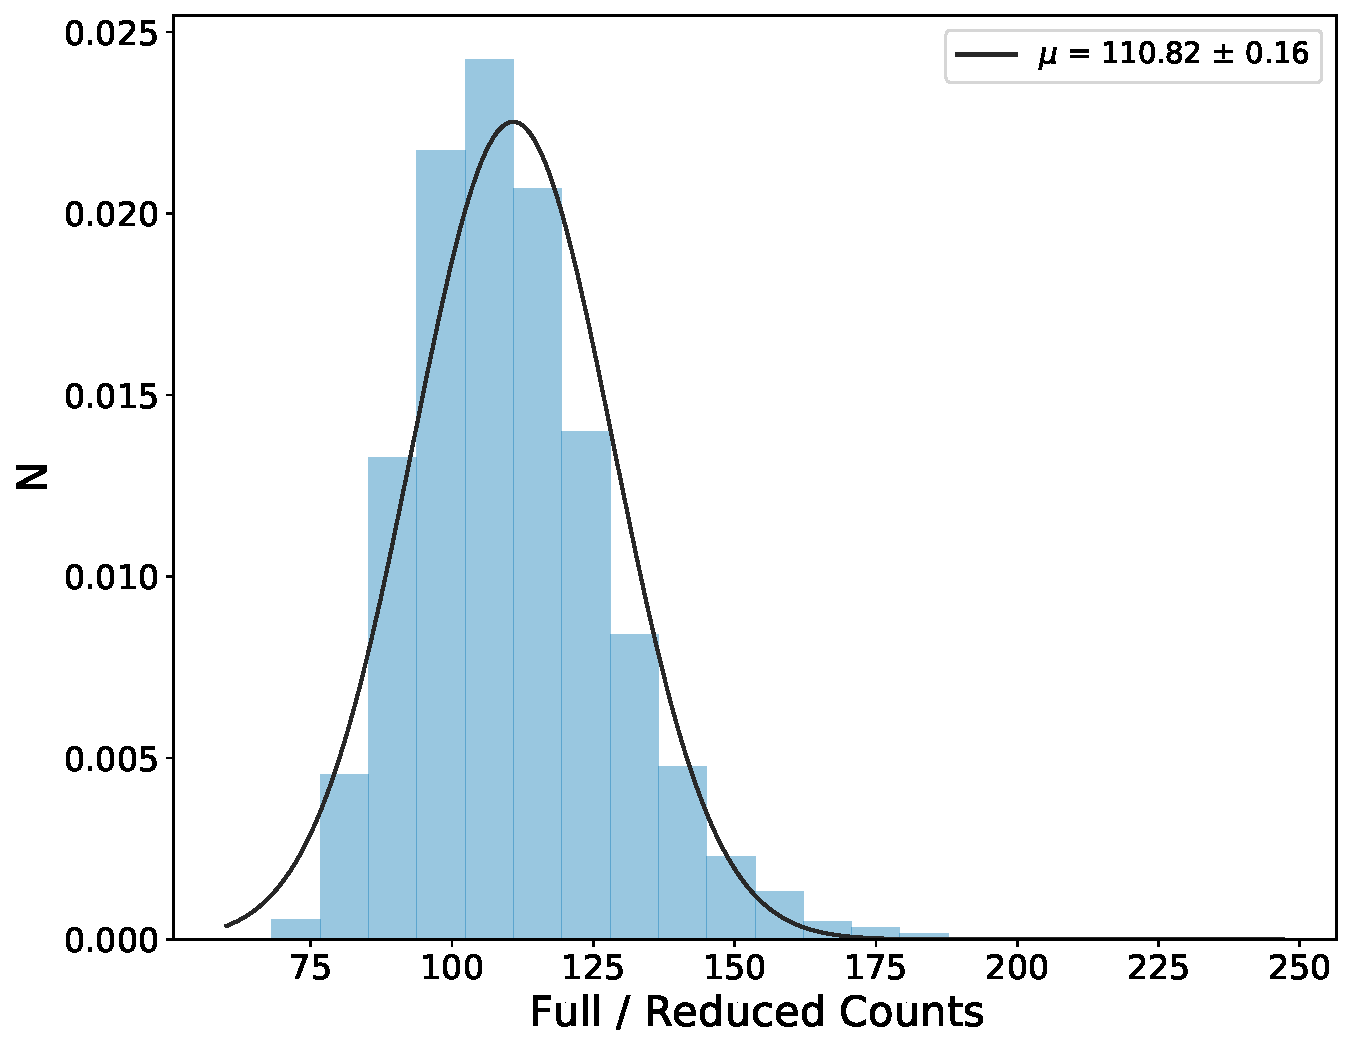
\includegraphics[width=0.44\columnwidth]{coinc_reduction_factor.pdf}
		\label{fig:rc2}} \\
	
	\caption{(a) Comparison of the reduced coincidences stored locally (orange) and as events data in the HiSPARC server (blue). (b) Distribution of the ratio of the full and reduced coincidence rates.}
	\label{fig:reduced_coincidences}
\end{figure}

The mean value of the Poisson distribution of these coincidence data is $\sim 44$~counts/min ($\sim 0.73 \, \upmu/\mathrm{s}$), which is a reduction by a factor of $\sim 110$ from the full coincidences data. We can see from Figure~\ref{fig:reduced_coincidences} that both the data stored locally (reduced coincidences) and the data sent to the \gls{hisparc} server (events) are in agreement, with only the realisation of the noise being different between the data. The \gls{hisparc} data acquisition software features a pre-trigger window (duration: $1 \, \upmu\mathrm{s}$), coincidence window (duration: $1.5 \, \upmu\mathrm{s}$), and a post-trigger window (duration: $3.5 \, \upmu\mathrm{s}$). The duration of these coincidence windows means that any delay on the order of $\sim 10$~ns is small, and does not effect the ability of the data acquisition software to record the data from the external trigger. This verifies that the locally stored reduced coincidences data and the events data stored in the \gls{hisparc} sever are measuring the same signal. With a count rate of count rate of $\sim 0.73 \, \upmu/\mathrm{s}$, the Poisson noise is on the same order of magnitude as the signal.


To understand the noise properties of this new configuration we investigated the random noise which is induced by random/spurious counts between both \glspl{pmt} and do not coincide with the passage of a muon. This was achieved by adding a delay in the signal between the two \glspl{pmt}, to ensure any coincident triggers were not due to true coincidences from the passage of a muon. By adding additional cables to the output from one \gls{pmt}, a delay of $\sim 120$~ns was added between the two signals. The \gls{fwhm} of a typical pulse from the \glspl{pmt} is $\sim$~25~ns, and the total duration from beginning-to-end is on the order of 100~ns \citep{van_dam_hisparc_2020}, therefore the $\sim 120$~ns delay was sufficient to remove true coincidences from the observations.

The delay was added between the two PMTs for around a week and the time series of the coincidences are shown in Figure~\ref{fig:random_coinciences}. We can see that the noise is nominally $\sim 1$~count/minute.

\begin{figure}[ht!]
	\centering
	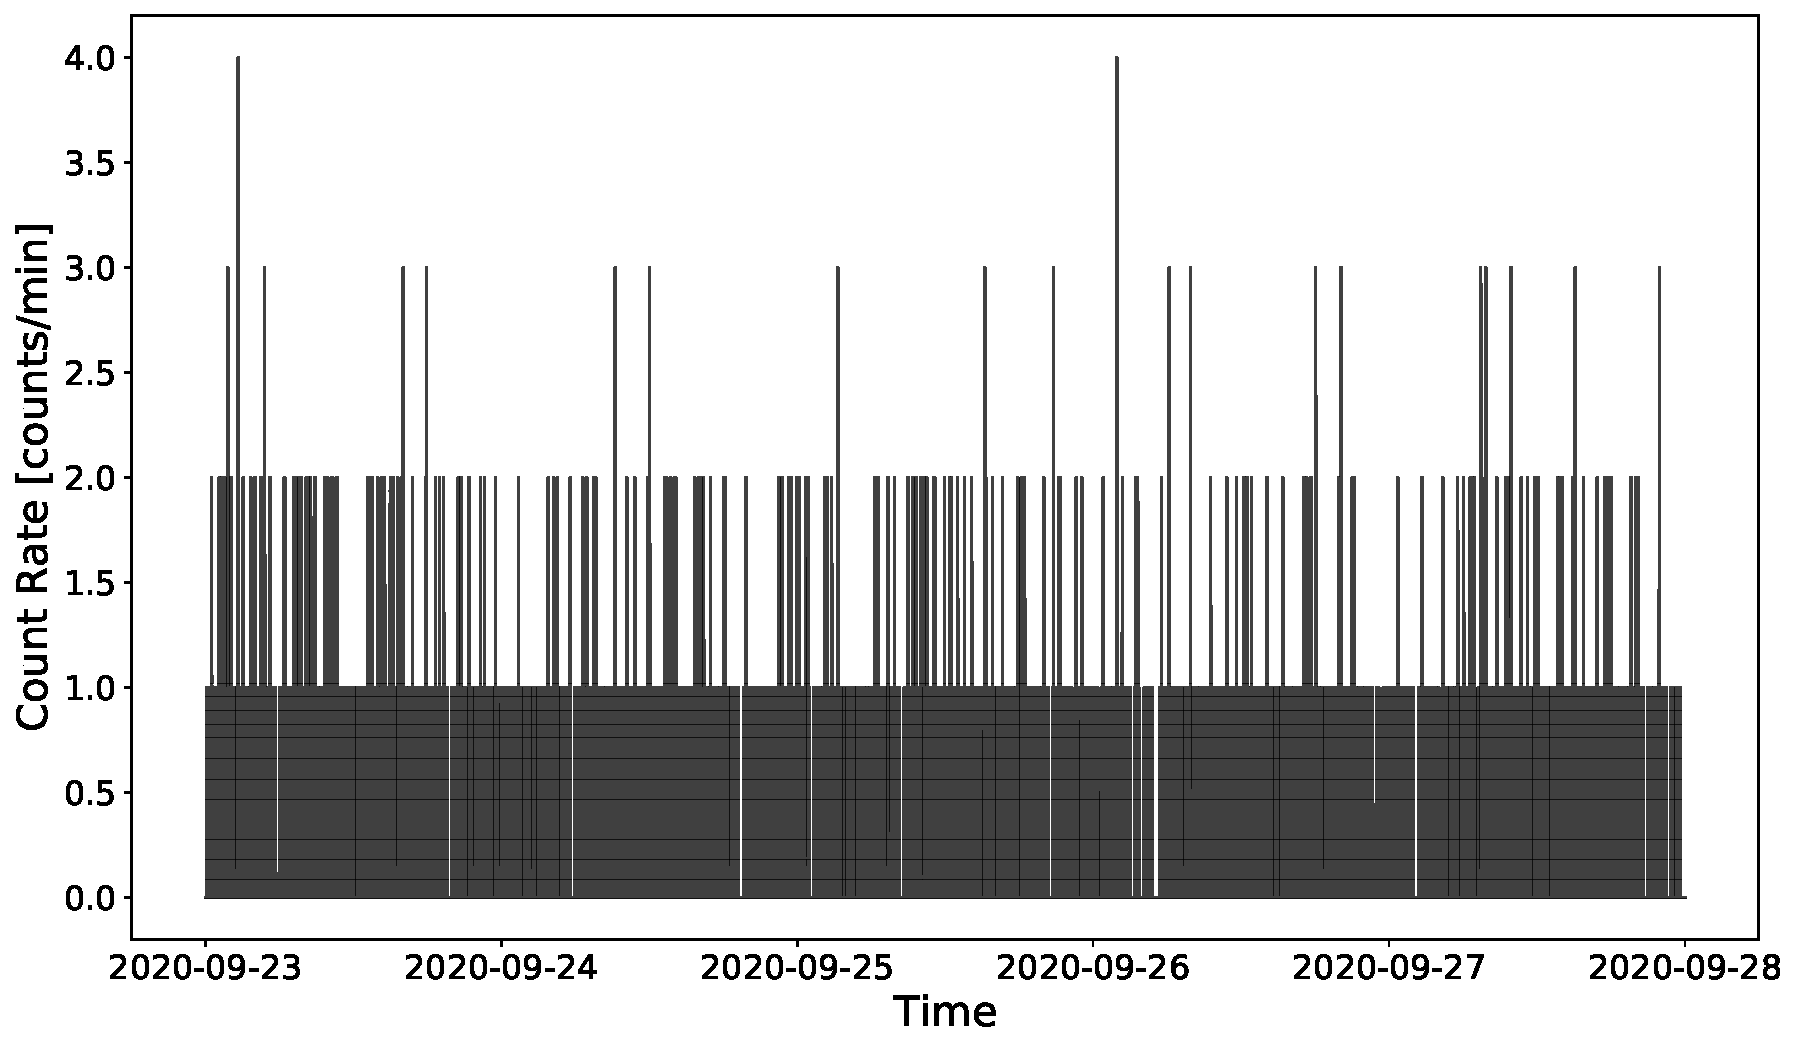
\includegraphics[width=\columnwidth]{random_noise_timeseries.pdf}
	\caption{Time series of random coincidences data...}
	\label{fig:random_coinciences}
\end{figure}

We know the noise must follow a Poisson distribution, therefore we aimed to quantify the mean value of the noise. The noise was sampled to determine the mean of the Poisson distribution using the {\verb pymc3 } \gls{nuts} extension to a \gls{hmc} sampling algorithm \citep{salvatier_probabilistic_2016}. Convergence was interrogated using the $\widehat{R}$ diagnostic factor using the criteria that chains did not converge if $\widehat{R} > 1.01$. The distribution of the random coincidences is shown in Figure~\ref{fig:random_coinciences_dist}

\begin{figure}[ht!]
	\centering
	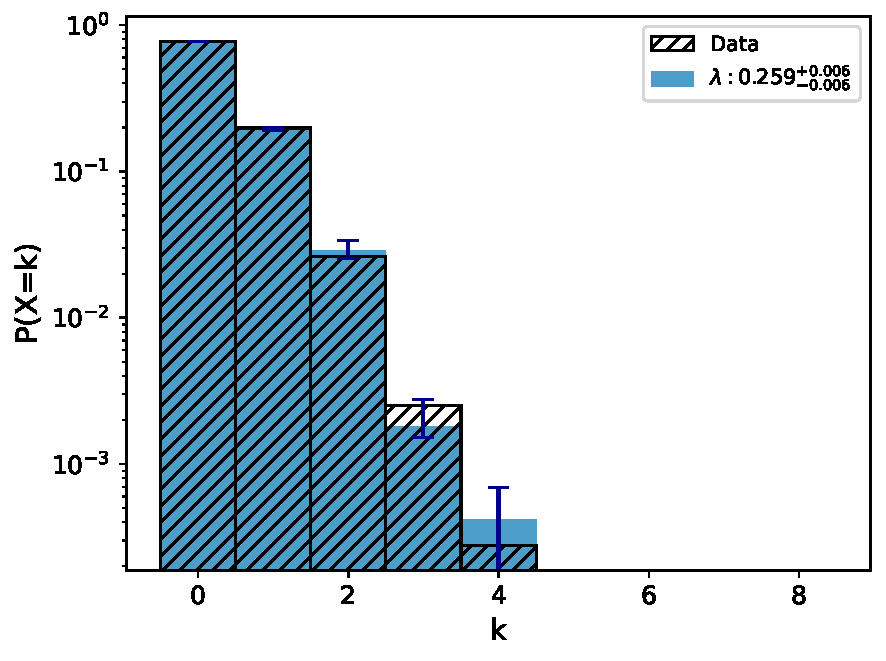
\includegraphics[width=0.9\columnwidth]{random_noise_fitted_poisson.pdf}
	\caption{Distribution of random coincidences data... and Poisson distribution of the random coincidences, along with the median posterior fitted mean of the sample...}
	\label{fig:random_coinciences_dist}
\end{figure}

The median value of the posterior distribution for the mean value of the Poisson distribution of random coincidence is $0.259 \pm 0.006$~counts/min, where the uncertainties represent the $68 \%$ credible intervals either side of the median. This represents a small noise; under this Poisson likelihood function the probability of no noise is $\sim 77 \%$, 1~count/minute is $\sim 20 \%$, and over 2~counts/minute is $< 3 \%$.

It is also important to note that in Figure~\ref{fig:random_coinciences}, there is no diurnal signal in the random noise. This shows that as the \gls{pmt} thermal noise increases around midday, which we see manifesting in the singles data, the increased thermal noise does not manifest in the spurious coincidences between both \glspl{pmt}. This is important as it highlights that in this stacked detector configuration we have maximised our ability to observe single muons whilst reducing the effects of diurnal, thermally induced noise.



%%%%%%%%%%%%%%%%%%%%%%%%%%%%%%%%%%%%%%%%%%%%%%%%%%%%%%%%%%%%%%%%%%%%%
%%%%%%%%%%%%%%%%%%%%%%%%%%%%%%%%%%%%%%%%%%%%%%%%%%%%%%%%%%%%%%%%%%%%%
\subsection{Comparison with Neutron Monitors}\label{sec:HS_14008_vs_Kiel}

[produce a comparison between this station's data and that for Kiel... show both in a plot and also do a correlation analysis!!]



%%%%%%%%%%%%%%%%%%%%%%%%%%%%%%%%%%%%%%%%%%%%%%%%%%%%%%%%%%%%%%%%%%%%%
\subsection{Single Station Space Weather Uses}\label{sec:HS_14008_single_sims}

[ simulations of \glspl{gle} using a model approximation using the results of the shape of \glspl{gle} from \citet{strauss_pulse_2017}. Modelled both the rise and the fall...]

[insert equation used to describe the GLE...]

[Refer to an appendix on the details of the model... but discuss that the properties were randomly selected and we forced the decay time to be > twice the rise time, to ensure the profile is similar to the standard of GLEs observed... Encorprotaed a signal which had a mean similar to that seen here, i.e. 80 muon~/~s... noise added for random fluctuations... randomly sampled the time series from poisson distriubtin...]

[Running several iterations it was possible to analyse the statistics of the resultant GLE and compare it to the background signal of the detector, without a GLE signal...]

[Insert example plot showing the stats tests, but mainly, show a new plot to show the background level and the level for the sims...]


\begin{figure}[ht!]
	\centering
	\subfloat[...]{
		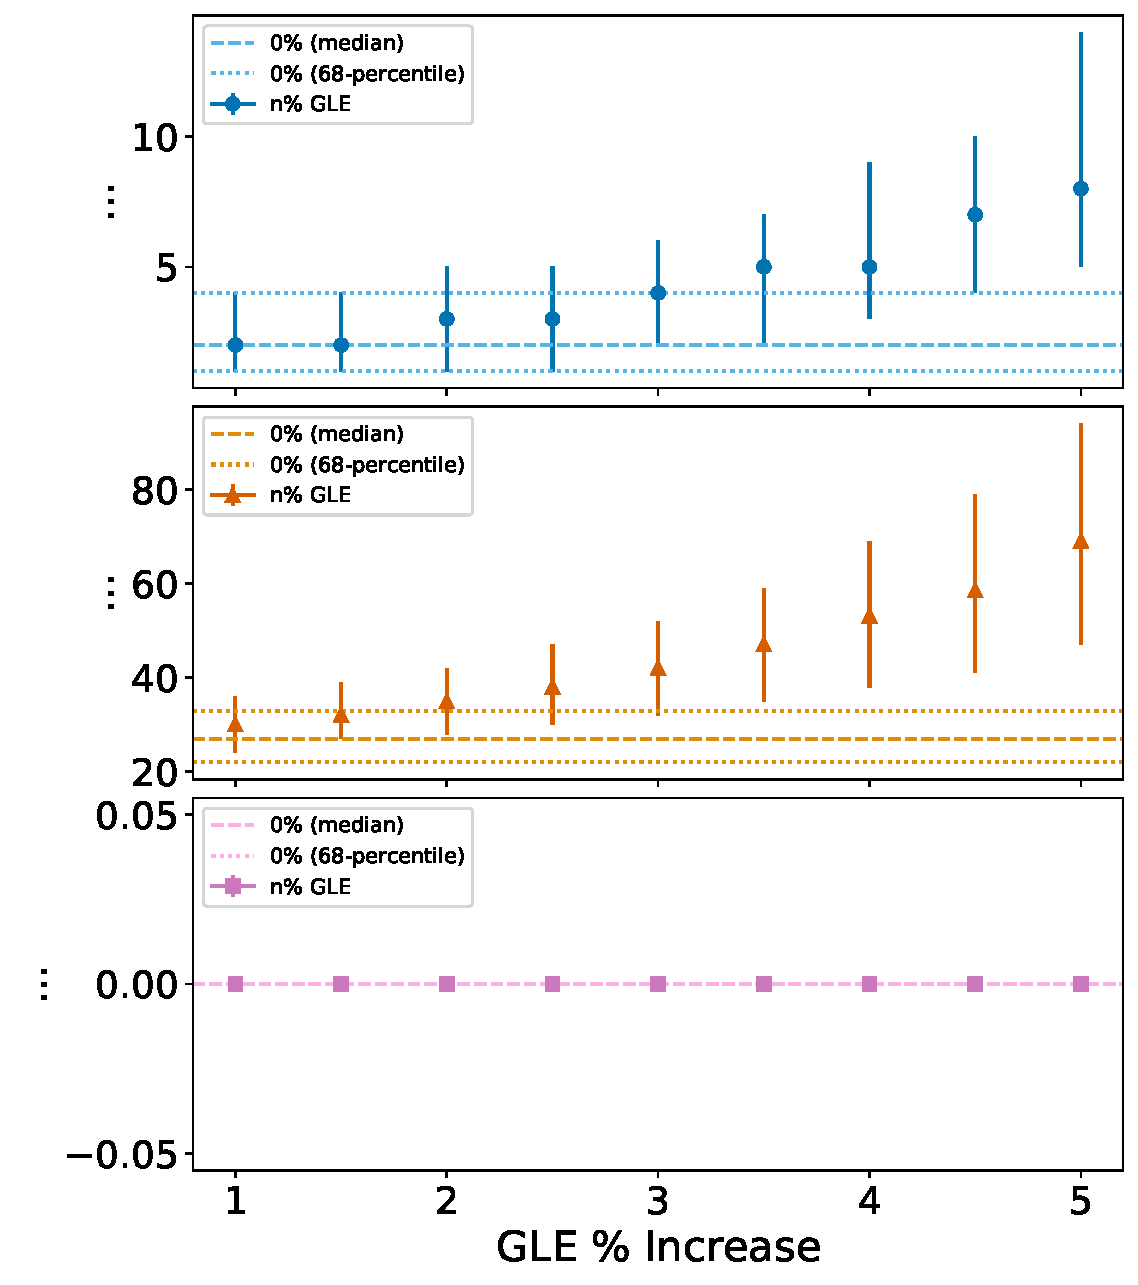
\includegraphics[width=0.48\columnwidth]{HS_14008_sims_plot_0rebin.pdf}
		\label{fig:1}}
	%\qquad
	\subfloat[...]{
		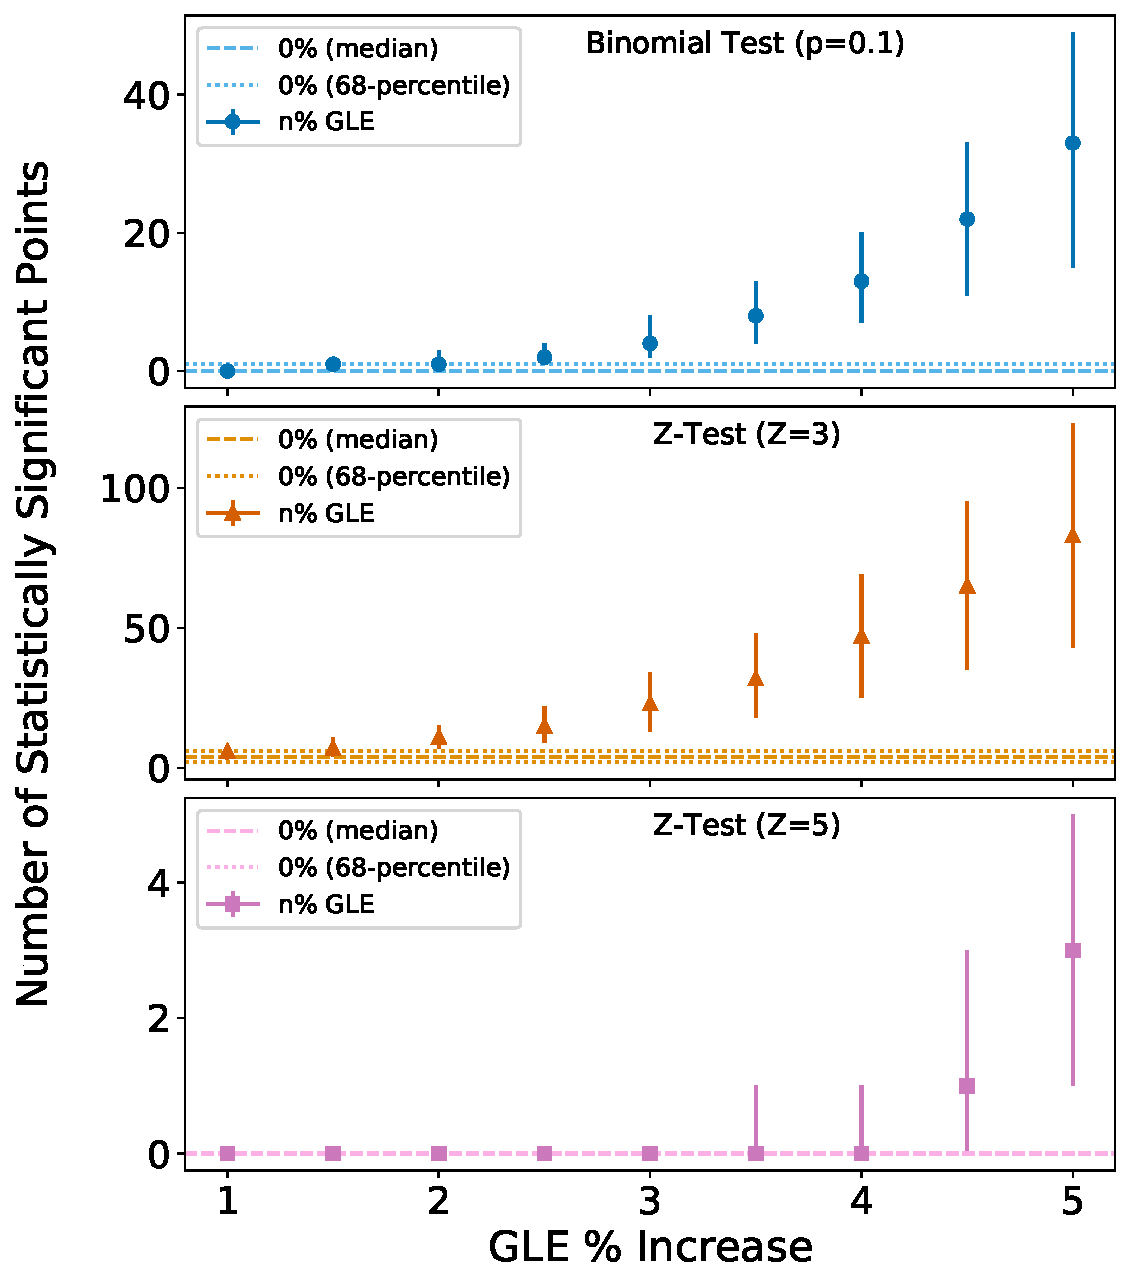
\includegraphics[width=0.48\columnwidth]{HS_14008_sims_plot_1rebin.pdf}
		\label{fig:2}} \\
	%\qquad
	\subfloat[...]{
		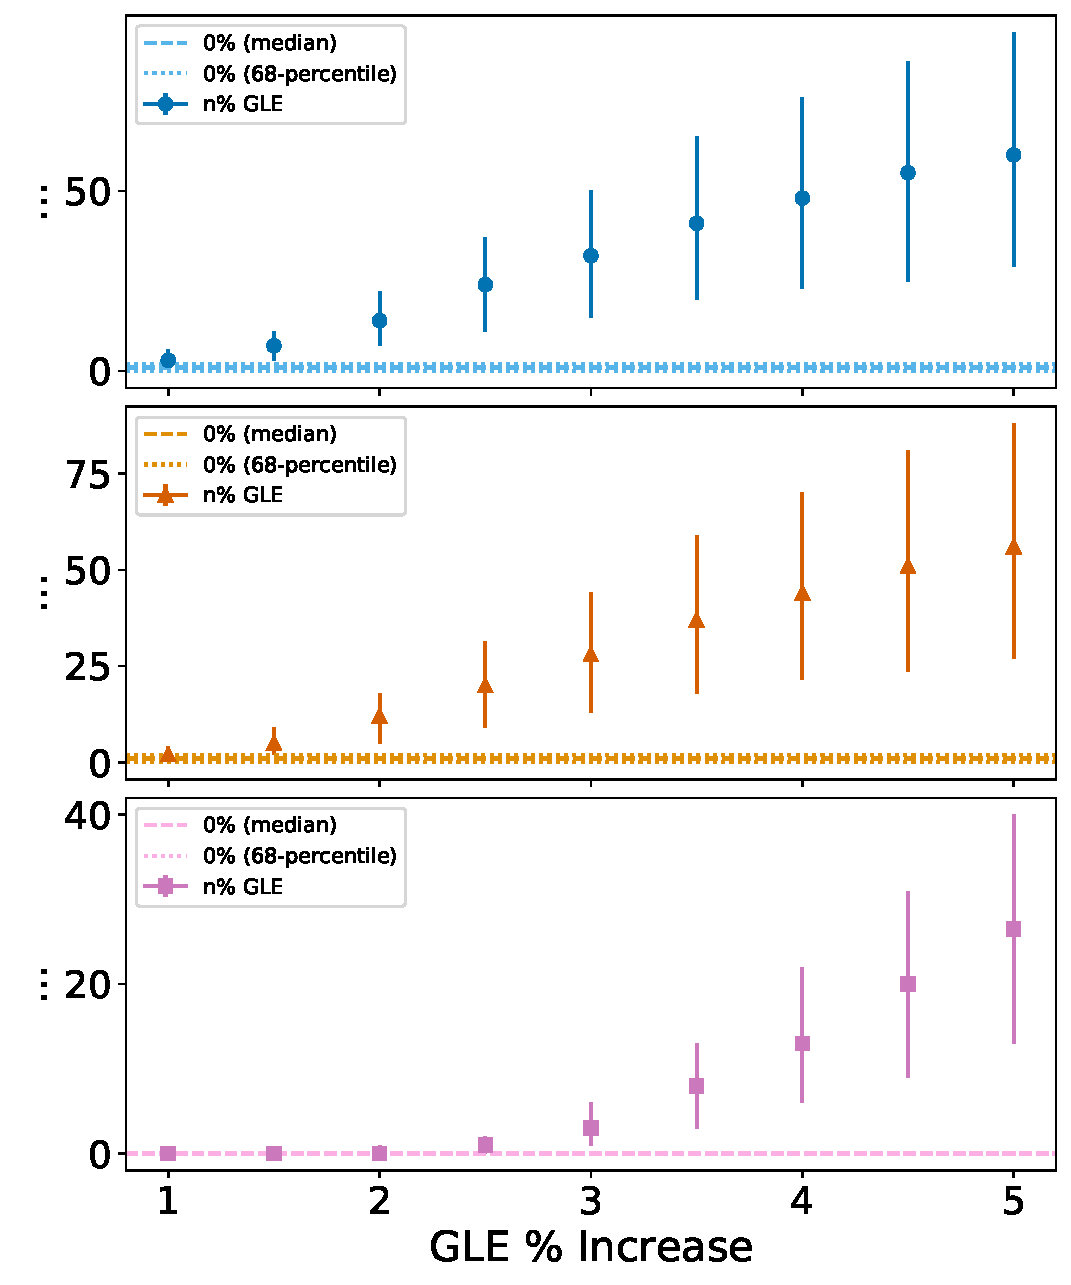
\includegraphics[width=0.48\columnwidth]{HS_14008_sims_plot_5rebin.pdf}
		\label{fig:3}} \\
	
	\caption{...}
	\label{fig:sims}
\end{figure}



%%%%%%%%%%%%%%%%%%%%%%%%%%%%%%%%%%%%%%%%%%%%%%%%%%%%%%%%%%%%%%%%%%%%%
\subsection{Multiple Station Space Weather Uses}\label{sec:HS_14008_multi_sims}



[Refer to an appendix on the details of the model again ...]

[Running several iterations...]

[Insert plot(s)...]


%%%%%%%%%%%%%%%%%%%%%%%%%%%%%%%%%%%%%%%%%%%%%%%%%%%%%%%%%%%%%%%%%%%%%
%%%%%%%%%%%%%%%%%%%%%%%%%%%%%%%%%%%%%%%%%%%%%%%%%%%%%%%%%%%%%%%%%%%%%
\section{Conclusions}\label{sec:HS_14008_conclusion}

We have presented a new \gls{hisparc} station configuration and investigated its performance as a monitor of space weather events...

...

...


We leave the reader with the following points:

\begin{enumerate}
	\item{}

	\item{}
	
	\item{}
\end{enumerate}